\documentclass[letterpaper,twocolumn]{article}

\usepackage{bigdelim}
\usepackage{graphicx}
\usepackage[marginal]{footmisc}
\usepackage{makecell}
\usepackage{multirow}
\usepackage{pifont} % For checkmarks in tab:nat-matching.
\usepackage{titling}
\usepackage{url}
\usepackage[table]{xcolor}

\usepackage[textsize=footnotesize]{todonotes}\setlength{\marginparwidth}{1.5cm}

% Better look for citations that include a section reference like \cite[\S 3]{foobar}.
\usepackage{cite}
\renewcommand{\citemid}{~}

% Load hyperref after other packages.
\usepackage[pdfa,hidelinks,pdfusetitle,pdfcreator={},pdfproducer={}]{hyperref}
\urlstyle{same}
\def\sectionautorefname{Section}
\def\subsectionautorefname{Section}

\usepackage{usenix-2020-09}

% Disable metadata for reproducible PDF.
% https://tex.stackexchange.com/a/313605
\usepackage{ifpdf}
\ifpdf
\pdfinfoomitdate=1
\pdftrailerid{}
\pdfsuppressptexinfo=-1
\fi

% Change URL line breaking preferences.
% http://mirrors.ctan.org/macros/latex/contrib/url/url.pdf §5.2 Changing linebreaks
% The considerations here are:
% 1. We must be able to break the URLs for Nasr2020a and uproxy-design-doc,
%    which have a path component that is longer than the line width but which
%    contains hyphens.
% 2. The URL for Barradas2020a looks much better if it is broken after a slash,
%    rather than after the hyphen in the hostname.
% 3. GitLab URLs in footnotes that end in #note_XXXXXXX look bad if broken
%    immediately after the '#'.
% \UrlBreaks have a lower penalty than \UrlBigBreaks; i.e., TeX will prefer to
% break lines at \UrlBreaks if possible, and only break at \UrlBigBreaks if
% necessary. We prefer to break at slashes only (which takes care of
% considerations 2 and 3), but will break at a hyphen when there is no slash
% available (which does consideration 1).
\def\UrlBreaks{\do-}
\def\UrlBigBreaks{\do/}

\hyphenation{Web-RTC}
\hyphenation{Web-Exten-sion}
\hyphenation{Java-Script}
\hyphenation{uProxy}
\hyphenation{off-line}
\hyphenation{mac-OS}
\hyphenation{Mull-vad}

% Highlight the first usage or definition of a technical term.
% Like the firstterm element in DocBook: https://tdg.docbook.org/tdg/5.2/firstterm.html.
\newcommand{\firstterm}[1]{\textit{#1}}

% Use a smaller font size for footnotes that consist entirely of a URL, so URLs like
% https://bugs.torproject.org/tpo/anti-censorship/pluggable-transports/snowflake/XXXXX
% fit in one line.
\setlength{\footnotemargin}{1.5ex}
\newlength{\urlfootnotesize}
\setlength{\urlfootnotesize}{6.5pt}
\newcommand{\urlfootnote}[1]{\footnote{
\raggedright\hangindent\footnotemargin%
\fontsize{\urlfootnotesize}{\urlfootnotesize}\selectfont%
\url{#1}
}}

\begin{document}

\date{}

\title{\Large\bf Snowflake, a censorship circumvention system\\using temporary WebRTC proxies\\\strut\large (Draft \today)}

\author{%
{\rm Cecylia Bocovich}%
\and
{\rm Arlo Breault}%
\and
{\rm David Fifield}%
\and
{\rm Serene}%
\and
{\rm Xiaokang Wang}%
}
\renewcommand{\maketitlehookc}{\centering\normalsize Authors are listed alphabetically.}

\maketitle

\begin{abstract}
Snowflake is a system for circumventing Internet censorship.
Its blocking resistance comes from
the use of numerous, ultra-light, temporary proxies (``snowflakes''),
which accept traffic from censored clients using peer-to-peer WebRTC protocols
and forward it to a centralized bridge.
The temporary proxies are simple enough to be implemented in JavaScript,
in~a web page or browser extension,
making them much cheaper to run than
a traditional proxy or VPN server.
The large and constantly changing pool
of proxy addresses resists enumeration and blocking by a censor.
The system is built on the assumption
that proxies may appear or disappear at any time:
clients discover live proxies dynamically
using a secure rendezvous protocol;
when an \mbox{in-use} proxy goes offline,
its client switches to another on the fly,
invisibly to upper network layers.

Snowflake has been deployed with success
in Tor Browser and Orbot for several years.
It has been a significant circumvention tool
during high-profile network disruptions,
including in Russia in~2021 and Iran in~2022.
In this paper, we explain the composition of Snowflake's many parts,
give a history of deployment and blocking attempts,
and reflect on implications for circumvention generally.
\end{abstract}

% General references:
%   https://keroserene.net/snowflake/technical/#history
%   https://www.bamsoftware.com/papers/thesis/#chap:snowflake

\section{Introduction}
\label{sec:intro}

Snowflake is a censorship circumvention system,
a~system to enable network communication
despite interference by a censor.
Its blocking resistance comes from a large pool
of low-cost, temporary proxies
that varies over time
and offers a censor no fixed target for blocking.
The core research purpose of this paper
is to investigate experimentally to what extent
a circumvention system that makes the tradeoffs Snowflake does
can be effective against contemporary censors.
We~will present the design of the system,
listing the many challenges of circumvention
and showing how Snowflake addresses them.
We~will explain how Snowflake solves the technical challenge
of providing a good user experience
when proxies are individually unreliable.
We~will document the reactions of national censors
through case studies in
Russia, Iran, China, and Turkmenistan
over more than three years of deployment.
On~the way we will provide quantitative evaluations
of various facets of the system,
including the number of clients served,
and the size and composition of the proxy pool.

Censorship circumvention systems may
be characterized on multiple axes.
Some systems imitate a common network protocol;
others try
not to look like any protocol in particular.
Some distribute connections over numerous proxy servers;
others concentrate on a single proxy
that is, for one reason or another, difficult for a censor to block.
What all circumvention systems have in common
is that they strive to increase the \emph{cost}
to the censor of blocking them---whether that cost be in
research and development, human resources, and hardware;
or in the inevitable overblocking that results
when a censor tries to selectively block
some connections but not others.
On~the spectrum of imitation to randomization,
Snowflake falls on the side of imitation;
on the scale of diffuse to concentrated, it is diffuse.
Snowflake's defining characteristic is that it
pushes the idea of distributed, disposable
proxies to an extreme.

WebRTC is a suite of protocols
intended for real-time communication applications
on the web~\cite{rfc8825}.
Video and voice chat are typical applications.
Snowflake exchanges WebRTC data formats
in the course of establishing a connection,
and uses WebRTC protocols to traverse of NAT (network address translation)
and to connect clients and proxies.
Crucially for Snowflake, WebRTC APIs
are available to JavaScript code in web browsers,
meaning it is possible to implement a proxy
in a web page or browser extension.
WebRTC is also usable outside a browser,
which is how we implement the Snowflake client program
and alternative, command line--based proxies.

As~is usual in circumvention research,
we assume a threat model in which
\firstterm{clients} reside in a network
controlled by a \firstterm{censor}.
The censor has the power to inspect and interfere with
traffic that crosses the border of its network;
typical real-world censor behaviors include
inspecting IP addresses and hostnames,
checking packet contents for keywords,
blocking IP addresses, and injecting false DNS responses
and TCP RST packets.
The client wants to communicate with some
\firstterm{destination} outside the censor's network,
possibly with the aid of third-party \firstterm{proxies}.
The censor is motivated to block the contents
of the client's communication, or the destination itself.
The censor knows of the possibility of circumvention,
and therefore seeks to block not only direct communication with the destination,
but also indirect communication by way of a proxy or circumvention system.
Circumvention is accomplished when the client
can reliably reach any proxy,
because a proxy, being outside the censor's control,
can then forward the client's communication to any destination.
(In Snowflake, we separate the roles of temporary \firstterm{proxies}
and a stable long-term \firstterm{bridge}, but the idea is the same.)
The censor derives benefit
from permitting some forms of network access:
it~cannot trivially ``win''
by shutting down all communication,
but must be selective in its blocking decisions,
in order to optimize some objective of its own.
The art of censorship circumvention is
forcing the censor into a dilemma
of~overblocking or underblocking,
by making circumvention traffic difficult to distinguish
from traffic that the censor prefers not to block.

Snowflake originates in two earlier projects:
flash proxy and uProxy.
% https://lists.torproject.org/pipermail/tor-dev/2016-January/010310.html "Snowflake is a webrtc pluggable transport inspired by flashproxy."
% https://keroserene.net/snowflake/technical/#1-introduction "It is inspired by and builds upon the previous work of Flashproxy. Snowflake is much like a hybrid of previous Pluggable Transports..."
Flash proxy~\cite{Fifield2012a}, like Snowflake, used
untrusted temporary JavaScript proxies in web browsers
forwarding to a central bridge,
but the link between client and proxy was WebSocket
rather than WebRTC,
which was then an emerging technology.
Flash proxy was deployed
% 2013: https://blog.torproject.org/combined-flash-proxy-pyobfsproxy-browser-bundles
% 2016: "Remove Flashproxy from Tor Browser" https://bugs.torproject.org/17428#note_2203210
from 2013 to~2016,
but never saw much use,
probably because WebSocket,
which lacks the built-in NAT traversal of WebRTC,
required clients to do complicated port forwarding.
% https://gitlab.torproject.org/legacy/trac/-/wikis/doc/PluggableTransports/FlashProxy/Howto
% https://serene.cx/snowflake/#note-flashproxy "...one could say that uProxy and flashproxy are the ancestors of snowflake."
uProxy~\cite{uproxy}, in one of its early incarnations,
% "in one of its earlier incarnations": uProxy pivoted from friend proxies to cloud servers in 2016:
% https://web.archive.org/web/20161211194847/https://blog.uproxy.org/2016/02/get-access-24x7-through-your-own-uproxy.html
% and added support for proxying through Tor in 2016:
% https://lists.torproject.org/pipermail/tor-dev/2016-September/011489.html
pioneered the use of WebRTC proxies for circumvention.
uProxy's proxies were browser-based,
but its trust and deployment model was different
from flash proxy's and Snowflake's.
Censored clients would arrange, out of band,
for an acquaintance outside the censor's network
to run a proxy in their browser~\cite{uproxy-design-doc}.
% uProxy v1.2.5 Design Doc: https://docs.google.com/document/d/1t_30vX7RcrEGuWwcg0Jub-HiNI0Ko3kBOyqXgrQN3Kw
% "uProxy depends on leveraging existing trust relationships to to find and use a proxy."
A~personal trust relationship was necessary to prevent misuse,
since browser proxies fetched destination content directly---meaning
client activity would be attributed to the proxy,
and the proxy might inspect the client's traffic.
Clients did not change proxies on the fly.
uProxy supported protocol obfuscation:
its packets could be transformed to resemble something
other than WebRTC.
% https://github.com/uProxy/uproxy-obfuscators
This was possible because of
uProxy's implementation as a privileged browser extension
with access to real sockets.
Because Snowflake uses ordinary unprivileged APIs,
its WebRTC can only look like WebRTC;
on the other hand, for the same reason,
Snowflake proxies are easier to deploy.
Like flash proxy, uProxy was active in the years
2013--2016.
% 2013: Serene's 30C3 lightning talk on uProxy https://events.ccc.de/congress/2013/wiki/Static:Lightning_Talks#Day_3
% 2013–2016 contributions in uProxy-p2p: https://github.com/UWNetworksLab/uProxy-p2p/graphs/contributors

Among existing circumvention systems,
the one that is most similar to Snowflake is MassBrowser~\cite{Nasr2020a},
% reading group summary of MassBrowser https://github.com/net4people/bbs/issues/32
which offers
proxying though volunteer proxies, called buddies.
MassBrowser's architecture is similar to Snowflake's:
there is a centralized component that coordinates
connections between clients and buddies,
which corresponds to a piece in Snowflake called the broker;
buddies are similar to our proxies.
The~trust model is in between Snowflake's and uProxy's.
Buddies preferentially operate as one-hop proxies, as in uProxy,
but are not limited to proxying only for trusted friends.
To~deter misuse, buddies specify a policy of
what categories of content they are willing to proxy.
The buddy software is
not constrained by a web browser environment,
and can, like uProxy, use protocol obfuscation
on the client--buddy link.
% V-D: "We also implement traffic obfuscation to protect MassBrowser's traffic
% against traffic analysis attacks. Particularly, we have built a custom
% implementation of the obfsproxy Tor pluggable transport tailored to work with
% our MassBrowser implementation."
% VI-A: "MassBrowser uses a custom protocol over TCP/UDP for the communications
% between Clients and Buddies."

Other circumvention systems have used WebRTC,
though without Snowflake's focus on numerous proxies.
Protozoa~\cite{Barradas2020a}
% reading group summary of Protozoa https://github.com/net4people/bbs/issues/55
and Stegozoa~\cite{Figueira2022a}
demonstrate point-to-point covert tunnel over WebRTC,
the former by directly replacing encoded media
with its own ciphertexts,
the latter using video steganography.
Significantly, where Snowflake now uses WebRTC data channels,
Protozoa and Stegozoa use WebRTC media streams,
which may have advantages for blocking resistance.
We will say more on this point in \autoref{sec:fingerprinting}.
TorKameleon~\cite{Vilalonga2023a} is a WebRTC-based system
with the dual goals of resisting blocking
and complicating traffic correlation attacks.
It~uses a recent draft programming interface called
WebRTC Encoded Transforms
% "Editor's Draft" status as of 2023-12-12 https://w3c.github.io/webrtc-encoded-transform/
% https://developer.mozilla.org/en-US/docs/Web/API/WebRTC_API/Using_Encoded_Transforms
to support Protozoa-like
embedding of data within media streams,
without invasive browser modifications.
% Examples of Encoded Transforms in TorKameleon source code:
% https://github.com/AfonsoVilalonga/TorKameleon/blob/c6ef7116043dfd74701ddb62f38606e748faf84b/PT/WebRTC/Client/public/js/main.js#L225
%   const transformStream = new TransformStream({
% https://github.com/AfonsoVilalonga/TorKameleon/blob/c6ef7116043dfd74701ddb62f38606e748faf84b/PT/WebRTC/Client/public/js/modulators/addFrame.js#L8
%   if (encodedFrame instanceof RTCEncodedVideoFrame && enconding.length > 0) {
% Encoded Transforms (earlier called Insertable Streams) had been mentioned as a future possibility in Stegozoa:
% https://dl.acm.org/doi/pdf/10.1145/3488932.3517419#page=12
% Snowflake team's notes:
% 2023-02-24 "WebRTC Encoded Transform (or Insertable Streams) for media channels in Snowflake?" https://lists.torproject.org/pipermail/anti-censorship-team/2023-February/000284.html

% Very early versions of Lantern (circa 2014) used social network–based trusted proxies:
%   https://web.archive.org/web/20140326223853/http://techpresident.com/news/wegov/24455/why-remarkably-similar-circumvention-tools-uproxy-and-lantern-are-not-overkill
%   https://lists.torproject.org/pipermail/tor-dev/2014-March/006356.html "HOWTO use Lantern as a pluggable transport"
%   https://web.archive.org/web/20130831160152/https://www.youtube.com/watch?v=aiPkCugE-RY
%   https://web.archive.org/web/2oe_/http://wayback-fakeurl.archive.org/yt/aiPkCugE-RY
% But it wasn't WebRTC, so was less like Snowflake than uProxy was.
% I'll draw the line here, since even Tor bridges are "volunteer-operated" in a sense.

Our goal in this paper is to provide a realistic assessment of Snowflake,
neither to exaggerate its advantages,
nor disproportionately emphasize the limitations
of other systems.
Circumvention research is a cooperative enterprise,
and we recognize and support our colleagues who
design and maintain their own systems.
With Snowflake, we have tried to explore a different point in the design space,
and by this exploration widen the scope of effective circumvention techniques.
We~acknowledge that Snowflake will be a better choice in some
censorship environments and
worse in others; indeed,
one of the ideas we hope to convey
is that blocking resistance
can be meaningfully understood only in relation to particular censor
and its resources, costs, and motivations.

As~of February 2024, Snowflake supports an estimated 42,000 average concurrent users
% > library("tidyverse")
% > WANTED_FINGERPRINTS <- c(
%     "7659DA0F96B156C322FBFF3ACCC9B9DC01C27C73" = "snowman",
%     "5481936581E23D2D178105D44DB6915AB06BFB7F" = "snowflake-01",
%     "91DA221A149007D0FD9E5515F5786C3DD07E4BB0" = "snowflake-02"
%   )
% > read_csv("figures/users/userstats-bridge-transport-multi.csv") %>%
%     filter(transport == "snowflake" & fingerprint %in% names(WANTED_FINGERPRINTS)) %>%
%     filter(date < "2024-02-01") %>%
%     mutate(users = users / (coverage / pmax(num_instances, coverage))) %>%
%     group_by(date, transport) %>% summarize(users = sum(users, na.rm = TRUE), .groups = "drop") %>%
%     tail()
% # A tibble: 6 × 3
%   date       transport  users
%   <date>     <chr>      <dbl>
% 1 2024-01-26 snowflake 41763.
% 2 2024-01-27 snowflake 43015.
% 3 2024-01-28 snowflake 43146.
% 4 2024-01-29 snowflake 42820.
% 5 2024-01-30 snowflake 41927.
% 6 2024-01-31 snowflake 42281.
at an average total transfer rate of 3.5~Gbit/s,
which works out to around 38~TB of circumvention traffic per day.
% > library("tidyverse")
% > WANTED_FINGERPRINTS <- c(
%     "7659DA0F96B156C322FBFF3ACCC9B9DC01C27C73" = "snowman",
%     "5481936581E23D2D178105D44DB6915AB06BFB7F" = "snowflake-01",
%     "91DA221A149007D0FD9E5515F5786C3DD07E4BB0" = "snowflake-02"
%   )
% > options(width = 200)
% > userstats <- read_csv("figures/users/userstats-bridge-transport-multi.csv") %>%
%     filter(fingerprint %in% names(WANTED_FINGERPRINTS)) %>%
%     mutate(users = users / (coverage / pmax(num_instances, coverage)))
% > bandwidth <- read_csv("figures/users/bandwidth-multi.csv") %>%
%     filter(fingerprint %in% names(WANTED_FINGERPRINTS)) %>%
%     filter(coverage > 0) %>%
%     mutate(bytes = bytes / (coverage / pmax(num_instances, coverage))) %>%
%     pivot_wider(id_cols = c(date, fingerprint), names_from = c(type), values_from = c(bytes)) %>%
%     mutate(
%       good_read = read - `dirreq-read`,
%       good_write = write - `dirreq-write`,
%       good_avg = (good_read + good_write) / 2,
%       good_avg_bps = good_avg*8/86400,
%     )
% > left_join(userstats, bandwidth, by = c("date", "fingerprint")) %>%
%     # Subtract out the pro-rated fraction of non-snowflake transports (basically negligible).
%     group_by(date, fingerprint) %>%
%     mutate(across(c(read, write, `dirreq-read`, `dirreq-write`, good_read, good_write, good_avg), ~ .x * users / sum(users))) %>%
%     ungroup() %>%
%     filter(transport == "snowflake") %>%
%     filter(date < "2024-02-01") %>%
%     group_by(date) %>%
%     summarize(
%       date = last(date),
%       across(c(read, write, `dirreq-read`, `dirreq-write`, good_read, good_write, good_avg, good_avg_bps), sum, na.rm = TRUE)
%     ) %>%
%     mutate(
%       across(c(read, write, `dirreq-read`, `dirreq-write`, good_read, good_write, good_avg), scales::label_bytes(units = "auto_si", accuracy = 0.01)),
%       across(c(good_avg_bps), scales::label_number(scale_cut = scales::cut_si("bit"), accuracy = 0.01)),
%     ) %>%
%     arrange(date) %>% tail()
% # A tibble: 6 × 9
%   date       read     write    `dirreq-read` `dirreq-write` good_read good_write good_avg good_avg_bps
%   <date>     <chr>    <chr>    <chr>         <chr>          <chr>     <chr>      <chr>    <chr>
% 1 2024-01-26 35.81 TB 35.68 TB 11.10 GB      221.14 GB      35.79 TB  35.46 TB   35.63 TB 3.30 Gbit
% 2 2024-01-27 37.01 TB 36.90 TB 11.34 GB      234.62 GB      37.00 TB  36.67 TB   36.84 TB 3.41 Gbit
% 3 2024-01-28 38.55 TB 38.46 TB 11.58 GB      251.62 GB      38.54 TB  38.20 TB   38.37 TB 3.55 Gbit
% 4 2024-01-29 38.15 TB 38.06 TB 11.67 GB      252.27 GB      38.14 TB  37.80 TB   37.97 TB 3.52 Gbit
% 5 2024-01-30 37.57 TB 37.48 TB 11.89 GB      253.14 GB      37.56 TB  37.23 TB   37.39 TB 3.46 Gbit
% 6 2024-01-31 38.31 TB 38.19 TB 10.87 GB      226.36 GB      38.30 TB  37.97 TB   38.13 TB 3.53 Gbit

\section{How it works}
\label{sec:mechanics}

\begin{figure*}[t]
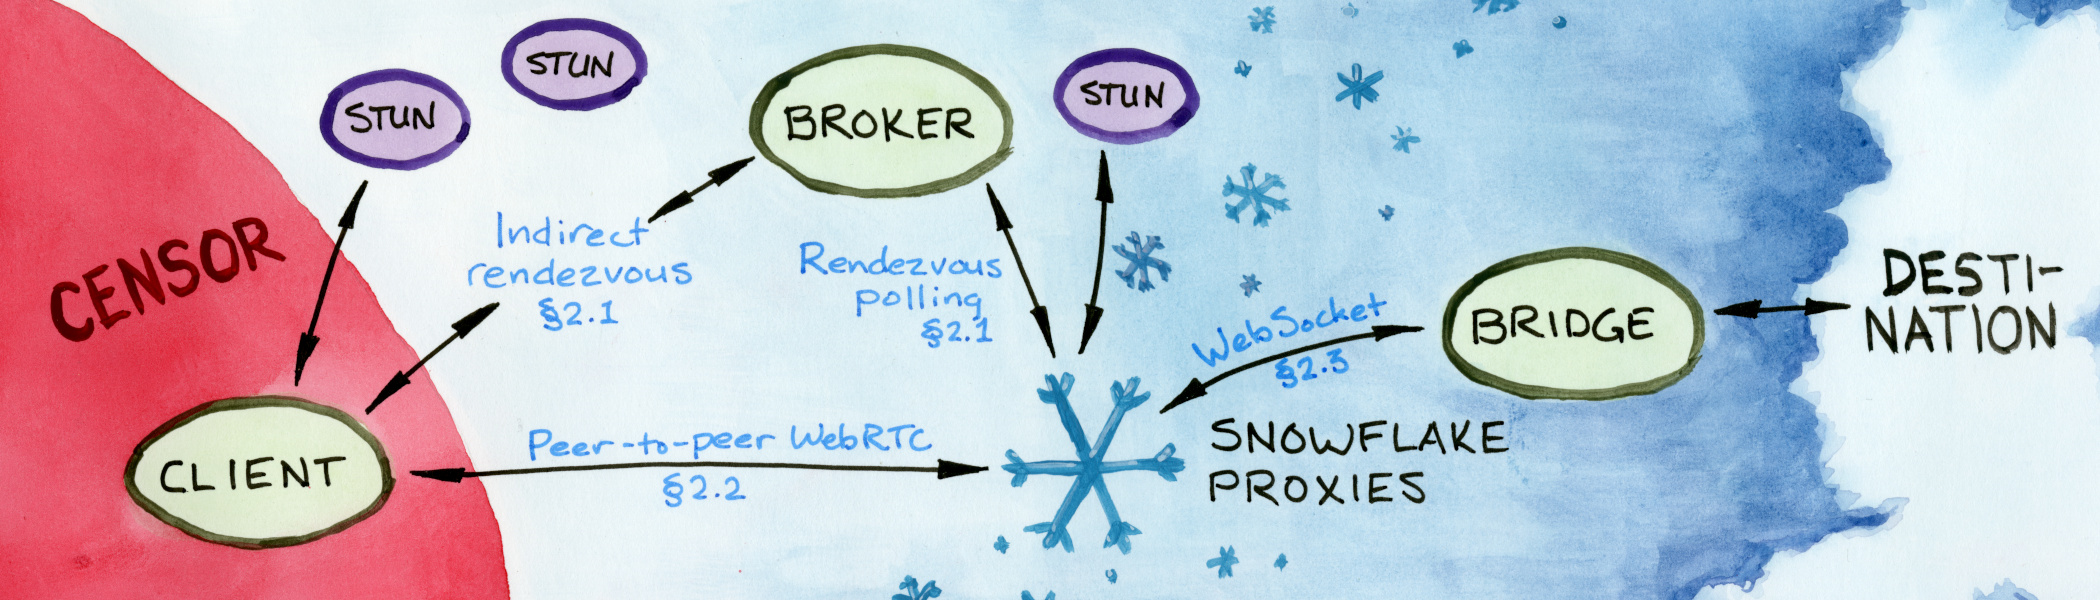
\includegraphics{figures/architecture/architecture.jpg}
\caption{
Architecture of Snowflake.
The client contacts the broker through a special rendezvous channel with high blocking resistance.
The broker matches the client with one of the proxies that are currently polling.
The client and proxy connect to one another using WebRTC.
The proxy connects to the bridge,
then begins copying traffic in both directions.
If~the proxy disappears,
the client does another rendezvous
and resumes its session with a new proxy.
}
\label{fig:architecture}
\todo[inline]{Make this graphic depict STUN servers and indirect rendezvous.}
\end{figure*}

A~Snowflake proxy connection proceeds in three phases.
First, there is rendezvous, in which a client
indicates its need for circumvention service
and is matched with a temporary proxy.
Rendezvous is facilitated by a central server called the broker.
Then, there is connection establishment,
where the client and its proxy connect to each other
with WebRTC, using information exchanged during rendezvous.
Finally, there is data transfer,
where the proxy transports data
between the client and the bridge.
The bridge is responsible for directing the client's traffic
to its eventual destination
(in~our case, by feeding it into the Tor network).
\autoref{fig:architecture} illustrates the process.

These phases repeat as needed, as temporary proxies come and~go.
Proxy failure is not an abnormal condition---it~happens whenever
a proxy is running in a browser that is closed, for example.
A~client builds a circumvention session over
a sequence of proxies, switching to a new one
whenever the current one stops working.
State variables stored at the client and the bridge
let the session pick up where it left off.
The change of proxies is invisible to the applications using Snowflake
(except for a brief delay for another rendezvous).
The Snowflake client presents an abstraction of one uninterrupted connection.

It~does not avail a censor to block the broker or bridge,
because Snowflake clients never contact either one directly.
Clients reach the broker over an indirect rendezvous channel.
Access to the bridge is always mediated by a temporary proxy.

\subsection{Rendezvous}
\label{sec:rendezvous}

A~session begins with the client sending a rendezvous message to the broker.
An~ambient population of proxies
constantly polls the broker to check for clients in need of service.
The broker matches the client with an available proxy,
taking into account factors like NAT compatibility.
% NAT type is currently the only constraint:
% matchSnowflake https://gitlab.torproject.org/tpo/anti-censorship/pluggable-transports/snowflake/-/blob/9edaee65470a1483bbdbe984e5e15a885f1e95d2/broker/ipc.go#L236
% But protocol versions may become a consideration in the future:
% "Analysis of speed deficiency of Snowflake in China, 2023 Q1" https://bugs.torproject.org/tpo/anti-censorship/pluggable-transports/snowflake/40251#note_2903271

The client's rendezvous message
% ClientPollRequest https://gitlab.torproject.org/tpo/anti-censorship/pluggable-transports/snowflake/-/blob/9edaee65470a1483bbdbe984e5e15a885f1e95d2/common/messages/client.go#L64
is a bundle of data that the broker will need in order to match the client with a proxy,
and the proxy will need in order to connect to the client.
The most important part of the rendezvous message is a
Session Description Protocol (SDP) \firstterm{offer}~\cite{rfc8839},
which contains the information needed for a WebRTC connection,
such as the client's external IP addresses
and cryptographic data to secure a later key exchange.
% Specifically, a certificate fingerprint: https://www.rfc-editor.org/rfc/rfc8122.html#section-5
The broker gives the client's offer to a currently polling proxy,
which sends back an SDP \firstterm{answer}
with its share of connection details.
The broker forwards the proxy's answer to the client,
and client and proxy then connect to one other directly.
In~WebRTC terms, this offer/\allowbreak answer exchange is called
``signaling''~\cite[\S 2.2]{rfc8825}, and here the broker acts as a signaling server.
To~gather the information for an SDP offer or answer,
clients and proxies communicate with third-party servers,
called STUN servers,
before contacting the broker.
We~will say more about how STUN is used in \autoref{sec:connection}.
Connecting to STUN servers is a normal part of WebRTC,
though there are fingerprinting considerations
that we cover in \autoref{sec:fingerprinting}.

Interaction with the broker uses a ``long-polling'' model,
depicted abstractly in \autoref{fig:rendezvous}.
Proxies poll the broker periodically,
making an ordinary HTTPS request.
The broker holds the connection open for a few seconds
to await a client rendezvous message.
If~none arrives, the broker sends a response that says ``no clients''
and the proxy goes to sleep until its next poll.
When a client does arrive,
the broker responds to the proxy's poll request
with the client's SDP offer.
The proxy re-connects to the broker to send back its SDP answer.
The broker sends the SDP answer to the client
and an acknowledgement to the proxy.
At~this point rendezvous is finished:
client and proxy have what they need to connect.

\begin{figure}
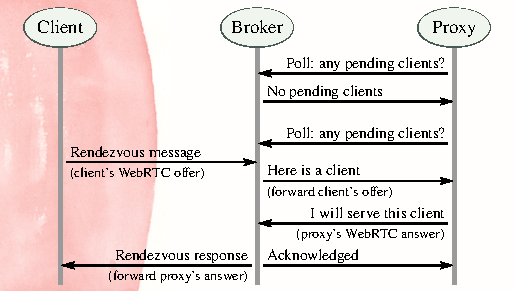
\includegraphics{figures/rendezvous/rendezvous}
\caption{
Information exchange in Snowflake rendezvous.
When the broker makes a match,
the proxy receives the client's SDP offer,
then re-connects to send back its SDP answer.
It~all happens during one round trip,
from the client's point of view.
Not shown is the indirect channel
the client must use to access the broker.
}
\label{fig:rendezvous}
\end{figure}

Proxies are free to connect to the broker directly,
because they are assumed to be uncensored.
But clients must use an indirect,
blocking-resistant channel,
because any direct connection with the broker
would be easily blocked by a censor.
What is needed, essentially,
is a miniature circumvention system to
bootstrap the full system.
But if clients have access to a bootstrap rendezvous method
that is good enough to reach the broker,
why is a more extensive circumvention system needed at all?
The answer is that the restricted scope of rendezvous
admits a wider range of solutions than general circumvention.
Techniques that would be too slow or expensive
for high-volume or interactive circumvention
may yet be suited to rendezvous,
because rendezvous happens infrequently
and transmits only small amounts of data.

The nice thing about rendezvous that it is modular and separable.
More than one method may be used,
and the methods need not have anything in common with the main system.
Anything that can be persuaded to convey a message
of about 1,500 bytes indirectly to the broker,
and return a response of about the same size,
may work as a Snowflake rendezvous module.
% "Broker: investigate non-domain-fronting secure client / proxy registrations" https://bugs.torproject.org/tpo/anti-censorship/pluggable-transports/snowflake/25594
% "DNS-based rendezvous for Snowflake" https://bugs.torproject.org/tpo/anti-censorship/pluggable-transports/snowflake/25874
% "Example: there is a chat bot (say, Telegram), that acts as a broker." https://bugs.torproject.org/tpo/anti-censorship/pluggable-transports/snowflake/25594#note_2823395
% Flash proxy email rendezvous would not work for Snowflake, because unidirectional.
% https://gitweb.torproject.org/flashproxy.git/tree/flashproxy-reg-email
% https://gitweb.torproject.org/flashproxy.git/tree/facilitator/fp-registrar-email
Snowflake now supports three rendezvous methods:

\begin{description}
\item[Domain fronting]
In~this method, the client does an HTTPS exchange with the broker
through an intermediary web service such as a content delivery network (CDN),
setting the externally visible hostname
(the TLS Server Name Indication, or SNI~\cite[\S 3]{rfc6066})
to a ``front domain'' different from the broker's.
The CDN routes the HTTPS request to the broker according to the
the HTTP Host header, which, under TLS encryption,
reflects the actual hostname of the broker~\cite{Fifield2015a}.
A~censor cannot easily block domain-fronted rendezvous
without also blocking unrelated connections to the front domain,
which should be selected to have high value to the censor.
The well-known drawback of domain fronting
is the high cost of CDN bandwidth,
but this is not a big problem
when it is used only for rendezvous.

\item[AMP cache]
AMP is a framework for web pages written in a restricted dialect of HTML.
Part of the framework is a free-to-use
cache server~\cite{amp-cache}.
The cache fetches AMP-conformant pages on demand,
making it effectively a restricted sort of HTTP proxy.
We~have a module that encodes rendezvous messages to conform to AMP requirements,
allowing them to be exchanged with the broker via the AMP cache.\urlfootnote{
% "AMP cache rendezvous"
https://gitlab.torproject.org/tpo/anti-censorship/pluggable-transports/snowflake/-/merge_requests/50
}
This rendezvous method is not easily blocked
without blocking the cache server as a whole.
It~still technically requires domain fronting,
because the AMP cache protocol normally exposes the
broker's hostname in the TLS SNI,
but it enlarges the set of usable intermediaries and front domains.

% "Snowflake rendezvous using Amazon SQS" https://bugs.torproject.org/tpo/anti-censorship/pluggable-transports/snowflake/26151
% "Deploy new SQS rendezvous method" https://bugs.torproject.org/tpo/anti-censorship/pluggable-transports/snowflake/40323
% https://gitlab.torproject.org/tpo/anti-censorship/pluggable-transports/snowflake/-/blob/38352b22ade217bd1372772b9cb69f8eff93e919/doc/rendezvous-with-sqs.md
\item[SQS (Simple Queue Service)]
Amazon SQS is a message queuing service designed for
communication between microservices.
Snowflake has the ability
(new at the time of this writing)
to use a message queue as a one-way communication channel.\urlfootnote{
https://gitlab.torproject.org/tpo/anti-censorship/pluggable-transports/snowflake/-/merge_requests/214
}
Clients write into a public queue, and the broker reads from~it.
Rendezvous response messages are sent back through
dynamically created, single-use queues.
Communication is indirect via SQS servers.
\end{description}

Rendezvous is not unique to Snowflake.
Other examples of rendezvous are
the DEFIANCE Rendezvous Protocol~\cite[\S 3]{Lincoln2012a},
the facilitator interaction in flash proxy~\cite[\S 3]{Fifield2012a},
and the registration proxy in Conjure~\cite[\S 4.1]{Frolov2019b}.
A~key property of Snowflake and the mentioned systems
is that their blocking resistance does not rely on preshared secret information.
Whatever information is needed to establish a circumvention session
is obtained dynamically at runtime.
This is in contrast to other systems in which,
before making a connection,
the client must acquire some secret,
such as an IP address or password,
through an out-of-band channel---and
blocking resistance depends on
keeping that information secret.
A~corollary of the no-secret-information property
is that an adversary is
at no special disadvantage in attacking the system.
There is no out-of-band channel which real clients have access to
but the censor does not.
The censor may pose as a client,
download the software,
study its network connections---and
the system must maintain its blocking resistance despite this.
The disadvantage of a separate rendezvous step
is that it is one more thing to get right.
Both the main circumvention channel
and the rendezvous must resist blocking:
the combination is only as strong as the weaker of the~two.

\subsection{Peer-to-peer connection establishment}
\label{sec:connection}

Now the client and the proxy connect to each other directly.
Even in the absence of censorship,
making a direct connection between two Internet peers is not always easy,
because of NAT (network address translation) and firewalls.
Snowflake clients and proxies alike run in diverse networks
with varying NATs and ingress policies.
Fortunately for us,
WebRTC is designed with this use case in mind,
and has built-in support for traversing NAT, in~the form of
ICE (Interactive Connectivity Establishment)~\cite{rfc8445},
a procedure for testing candidate pairs of peer network addresses
to find one that works.
ICE~makes use of third-party
STUN (Session Traversal Utilities for NAT)~\cite{rfc8489}
servers that, among other things,
enable a host to learn its external IP addresses.
The first part of ICE took place at the beginning of rendezvous,
when the client and proxy contacted STUN servers to gather
external address candidates and included them in their respective
SDP offer and answer.

There is no guarantee that two hosts will be able to make
a connection using the facilities of STUN alone.
Some address mapping and
filtering setups are simply incompatible.
In~such a case,
ICE would normally fall back to using
TURN (Traversal Using Relays around NAT)~\cite{rfc8656},
a~kind of UDP proxy.
Such a fallback would be problematic for Snowflake,
because the TURN relays themselves
would become a target of blocking by the censor.
% "Configure TURN servers for the proxy and/or client" https://bugs.torproject.org/tpo/anti-censorship/pluggable-transports/snowflake/25596
But Snowflake has an advantage most WebRTC applications do not.
Most WebRTC applications want to connect \emph{a particular} pair of peers,
whereas we are satisfied when a client can connect to \emph{any} proxy.
Snowflake clients and proxies self-measure their NAT type
and report it to the broker,
which takes NAT compatibility into account
and avoids cases that would require a fallback to TURN.

% "Investigate Snowflake proxy failures" https://bugs.torproject.org/tpo/anti-censorship/pluggable-transports/snowflake/33666#note_2595319
% "Okay here's a summary of what I've found: ..."

We condense the possible combinations of NAT and firewall features
that impact
a Snowflake client or proxy's
ability to make a peer-to-peer connection
into the following well-known variations:

% https://datatracker.ietf.org/doc/html/rfc3489#section-5
\begin{description}
\item[Full cone]
The same internal IP--port pair always maps to the same external port.
Any remote host may send a packet to an internal IP address and port by sending a packet to the
mapped external port.
\item[Restricted cone]
Like full cone,
but incoming packets
are allowed only if
there has recently been an outgoing packet
to the same remote IP address.
\item[Port-restricted cone]
Like restricted cone,
but incoming packets are allowed only if
there has recently been an outgoing packet
to the same remote IP--port pair.
\item[Symmetric]
The external port depends on both
the internal IP--port pair and the remote IP--port pair.
Incoming packets are allowed only if
there has recently been an outgoing
packet to the same remote address.
\end{description}

\begin{table}
\definecolor{Ycolor}{Gray}{14}
\definecolor{ncolor}{Gray}{13}
\newcommand{\Y}{\cellcolor{Ycolor}\ding{51}}
\newcommand{\n}{\cellcolor{ncolor}--}
\newcommand{\rotlabel}[1]{\rotatebox{30}{#1}}
% \vphantom is to make the labels take up vertical space;
% \rlap is so they don't expand the horizontal size of table columns.
\newcommand{\rot}[1]{\vphantom{\rotlabel{#1}}\rotlabel{\rlap{#1}}}
\centering
% Make normal cells taller by default.
\renewcommand{\arraystretch}{1.25}
% Tighten line spacing in \makecell cells.
\renewcommand\cellset{\renewcommand\arraystretch{0.8}\setlength\extrarowheight{0pt}}
\begin{tabular}{@{}rcccccl@{\hspace{0.5ex}}l@{}}
& % empty
\rot{No NAT} &
\rot{Full cone} &
\rot{Restricted cone} &
\rot{Port-restricted cone} &
\rot{Symmetric} &
&
\\
No NAT               & \Y & \Y & \Y & \Y & \Y & \multirow{3}{*}{\kern-\tabcolsep\kern0.5ex\footnotesize\(\left.\kern-\nulldelimiterspace\rule[-19pt]{0pt}{38pt}\right\}\)} & \multirow{3}{*}{\footnotesize\makecell[l]{unrestricted\\proxy}} \\
Full cone            & \Y & \Y & \Y & \Y & \Y & \\
Restricted cone      & \Y & \Y & \Y & \Y & \Y & \\
Port-restricted cone & \Y & \Y & \Y & \Y & \n & \multirow{2}{*}{\kern-\tabcolsep\kern0.5ex\footnotesize\(\left.\kern-\nulldelimiterspace\rule[-12pt]{0pt}{24pt}\right\}\)} & \multirow{2}{*}{\footnotesize\makecell[l]{restricted\\proxy}} \\
Symmetric            & \Y & \Y & \Y & \n & \n & \\[\dimexpr 0.5ex - \dimexpr 0.5\dimexpr\arraystretch\normalbaselineskip]
% \hfill hack to make \upbracefill work with colortbl:
% https://tex.stackexchange.com/questions/202138/upbracefill-filling-entire-tabular-cell-and-package-colortbl#comment474604_202143
                     & \multicolumn{4}{@{~}c@{~}}{\footnotesize\def\hfill{\hskip 0pt plus 1filll}\upbracefill} & \clap{\footnotesize\def\hfill{\hskip 0pt plus 1filll}\upbracefill} & \\
                     & \multicolumn{4}{c}{\footnotesize\makecell{unrestricted\\client}} & \clap{\footnotesize\makecell{restricted\\client}} \\
\end{tabular}
\caption{
Pairwise compatibility of NAT variants,
assuming the facilities of STUN alone
(no~fallback to TURN).
The incompatible cases,
which the broker tries to avoid when matching,
are when one peer's NAT is symmetric
and the other's is symmetric or port-restricted cone.
Note the asymmetry in what NAT variants are considered ``restricted''
in client and proxy.
}
\label{tab:nat-matching}
\end{table}

\autoref{tab:nat-matching}
shows the pairwise compatibility of NAT variations.
As~the incompatible cases always involve a symmetric NAT,
we further simplify matching by categorizing the variations into the two types
\firstterm{unrestricted} (works with most other NATs) and
\firstterm{restricted} (works only with more permissive NATs).
Unrestricted proxies may be matched with any client;
restricted proxies may be matched only with unrestricted clients.
The broker prefers to match unrestricted clients with restricted proxies,
% https://gitlab.torproject.org/tpo/anti-censorship/pluggable-transports/snowflake/-/blob/9edaee65470a1483bbdbe984e5e15a885f1e95d2/broker/ipc.go#L236
in~order to conserve unrestricted proxies
for the clients that need them.
Symmetric NAT is always considered restricted,
but port-restricted cone NAT differs
depending on the peer:
for proxies it is restricted, but
for clients it is unrestricted.
The asymmetric categorization is an approximation
to help conserve unrestricted proxies
for clients with symmetric NATs.
Though it creates the potential for an incompatible match,
we believe this to be uncommon in practice.
In~case of a connection failure,
clients re-rendezvous and try again.

To self-assess their NAT type,
clients use the NAT behavior discovery feature of STUN~\cite{rfc5780}.
% "Use STUN to determine NAT behaviour of peers" https://bugs.torproject.org/tpo/anti-censorship/pluggable-transports/snowflake/34129
% "Add utility to help user discover their NAT type" https://github.com/pion/stun/issues/8
Proxies cannot use the same technique,
because the necessary STUN features are not exposed
to JavaScript.
Instead,
we adapt a technique from MassBrowser~\cite[\S \mbox{V-A}]{Nasr2020a}
and run a centralized, always-on WebRTC testing peer
behind a simulated symmetric NAT.\urlfootnote{
% "Have a remote probe service to test snowflake proxy NAT compatability"
https://bugs.torproject.org/tpo/anti-censorship/pluggable-transports/snowflake/40013
}
Proxies try connecting to this peer:
if~the connection succeeds, the proxy's type is unrestricted;
otherwise it is restricted.
Clients and proxies retest their NAT type periodically,
to account for potential changes in their local networking environment.
If~a client or proxy is unable to determine its NAT type for some reason,
it reports the type ``unknown,''
which the broker conservatively treats as if it were restricted.

\begin{figure}
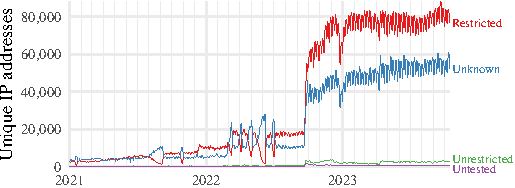
\includegraphics{figures/proxies/proxy-nat-type}
\caption{
Proxy NAT types, in unique IP addresses per day.
The places in 2021 and 2022
where ``Unknown'' displaced other types
were caused by operational problems with
the centralized NAT type testing peer.
% "Increase of 'unknown' NAT assignments by probetest since 2021-10-25" https://bugs.torproject.org/tpo/anti-censorship/pluggable-transports/snowflake/40071
% "Move snowflake-broker to a systemd based setup" https://bugs.torproject.org/tpo/anti-censorship/pluggable-transports/snowflake/40147
}
\label{fig:proxy-nat-type}
\end{figure}

\autoref{fig:proxy-nat-type}
shows that unrestricted proxies form
a relatively small fraction of the proxy population.
In~absolute terms, there are enough,
thanks in large part to the volunteers who run
the command-line
version of the Snowflake proxy
on networks unencumbered by NAT.
Though stable, long-term proxies go
somewhat against the ethos of Snowflake,
it~has proved useful, as a matter of practicality,
to~sacrifice a measure of address diversity
for better NAT compatibility in a common case.
We~can estimate how many tries it takes a client
to be matched with a proxy, on average,
by counting failed and successful rendezvous attempts at the broker,
under the assumption that clients repeat rendezvous attempts
until getting a match.
In~July 2023,
unrestricted clients almost always got a match on the first attempt,
while restricted clients needed an average of
1.07 attempts (standard deviation 0.05).
% > library(tidyverse)
% > read_csv("figures/proxies/client-match.csv") %>%
%     filter(date < "2024-02-01") %>%
%     group_by(month = format(date, "%Y-%m")) %>%
%     summarize(
%       unrestricted_n  = mean((matched_count + unrestricted_denied_count) / matched_count),
%       unrestricted_sd =   sd((matched_count + unrestricted_denied_count) / matched_count),
%       restricted_n    = mean((matched_count + restricted_denied_count) / matched_count),
%       restricted_sd   =   sd((matched_count + restricted_denied_count) / matched_count),
%       .groups = "drop"
%     ) %>% tail(10)
% # A tibble: 10 × 5
%    month   unrestricted_n unrestricted_sd restricted_n restricted_sd
%    <chr>            <dbl>           <dbl>        <dbl>         <dbl>
%  1 2023-04           1        0                   1.15       0.152
%  2 2023-05           1.00     0.00204             1.23       0.113
%  3 2023-06           1.00     0.0000834           1.23       0.0734
%  4 2023-07           1        0                   1.07       0.0498
%  5 2023-08           1        0                   1.02       0.0568
%  6 2023-09           1        0                   1.00       0.0148
%  7 2023-10           1.00     0.000000552         1.01       0.0137
%  8 2023-11           1        0                   1.00       0.00499
%  9 2023-12           1        0                   1.00       0.0121
% 10 2024-01           1        0                   1.01       0.0168

While the proxy is connecting to its client,
% "While": https://gitlab.torproject.org/tpo/anti-censorship/pluggable-transports/snowflake/40228
it also connects to the bridge.
This connection
uses WebSocket~\cite{rfc6455}, which
offers a TCP-like, client--server connection
layered on HTTPS.
The choice of protocol for the proxy--bridge link is arbitrary,
and could be changed
without affecting the rest of the system.
It does not need to be resist blocking,
it~just needs to be available to JavaScript code in web browsers.
WebRTC, for example, could be used for this link as well.

\subsection{Data transfer}
\label{sec:data-transfer}

No~complicated processing takes place at the proxy.
The main value of a Snowflake proxy is its IP address:
it~gives the client a peer to connect to that is not on the censor's address blocklist.
Having provided that,
the proxy assumes a role of pure data transfer.

Snowflake uses a stack of nested protocol layers.
We~will walk though the layers and describe the purpose of each.

\bigskip

\noindent
\begin{tabular}{@{}l@{\,}l@{}l@{\,}l}
UDP & \rdelim\}{3}{*} & \multirow{3}{5em}{WebRTC data channel} & \rdelim\}{3}{*}[\,ephemeral, per proxy]\\
DTLS \\
SCTP \\
KCP & \rdelim\}{2}{*} & \multirow{2}{*}{Turbo Tunnel} & \rdelim\}{3}{*}[\,persistent, per session] \\
smux \\
\multicolumn{3}{@{}l}{Tor protocol} \\
\multicolumn{4}{@{}l}{application streams} \\
\end{tabular}

\bigskip

\noindent
This is the stack for the client--proxy link,
which is the place where WebRTC is used, and which is
exposed to observation by the censor (\autoref{fig:architecture}).
The stack for the proxy--bridge link is the same,
but with WebSocket in place of the
WebRTC data channel at the top.
The layers marked ``ephemeral'' are skimmed off
and replaced as proxies come and~go.
The layers marked ``persistent'' are instantiated once
in each circumvention session,
hold long-term state,
and are end-to-end between client and bridge.

The connection between a client and its proxy is
a WebRTC data channel~\cite{rfc8831},
which provides a way to send arbitrary binary messages between peers.
A~data channel is its own stack of three protocols:
UDP for network transport,
DTLS (Datagram TLS)
for confidentiality and integrity, and
SCTP (Stream Control Transmission Protocol)
for delimiting message boundaries
and other features like congestion control.
Working UDP port numbers will have been discovered
using ICE in the previous phase.
The peers authenticate one another
at the DTLS layer using certificate fingerprints
that were exchanged during rendezvous~\cite[\S 5.1]{rfc8842}.

Data channels are well-suited to Snowflake's needs.
(The specification even lists circumvention as a use case~\cite[\S 3.2]{rfc8831}.)
But data channels are not the only option:
WebRTC also offers \firstterm{media streams}
for unreliable transport of real-time audio and video.
Which of these is used may be a fingerprinting vector.
We~will take up this topic in \autoref{sec:fingerprinting}.

If~clients only ever used one proxy,
a~WebRTC data channel alone would be sufficient.
But a Snowflake proxy might
disappear at any moment,
and when that happens, its data channel goes with~it.
If~the client was in the middle of a long download,
for example, it should be possible to resume the download
without interruption after rendezvousing with a new proxy.
For this we need a shared notion of session state that exists
at the client and the bridge, not tied to any temporary proxy.
A~lack of session continuity across proxy failures
had been an unsolved problem in flash proxy~\cite[\S 5.2]{Fifield2012a}.

We~adopt the
Turbo Tunnel design pattern~\cite{Fifield2020a}
and insert a userspace
session and reliability protocol
between the ephemeral proxy data channels
and the client's own application streams.\urlfootnote{
% "[anti-censorship-team] Turbo Tunnel in Snowflake"
https://lists.torproject.org/pipermail/anti-censorship-team/2020-February/000059.html
}
This part of the protocol stack
outlives any single proxy; it~belongs to
the client and the bridge.
Its primary function is to attach sequence numbers and acknowledgements
to packets of data,
so~that both ends know what parts of the data stream
need to be retransmitted after a temporary loss of proxy connectivity.
The client tags its traffic
with a random session identifier string that remains
consistent throughout a session,
which the bridge uses to index a map of session variables.
For the inner session layer we use a combination of
KCP~\cite{kcp} and
smux~\cite{smux}.
KCP provides reliability,
and smux detects the end of idle sessions and terminates them.
KCP and smux have shown their worth in other deployments,
and are easy to program,
but there is nothing about them on which we depend essentially.
Any other transport protocol that provides the necessary features
and can be implemented in userspace would~do,
such as QUIC, TCP, or (another layer~of) SCTP.
We~prototyped successfully with QUIC before deciding on KCP/\allowbreak smux.

% Not going to get into how we currently use reliable, ordered (TCP-like) data
% channels, but plan to switch to unreliable, unordered (UDP-like) data
% channels, a better fit for the underlying datagram-oriented Turbo Tunnel
% layer.
%
% "turn off reliable mode for WebRTC DataChannel" https://gitlab.torproject.org/tpo/anti-censorship/pluggable-transports/snowflake/-/merge_requests/109
% "Snowflake is currently using network resource in a so suboptimal way..." https://bugs.torproject.org/tpo/anti-censorship/pluggable-transports/snowflake/40251#note_2891751

One more protocol layer is needed inside the tunnel:
an~end-to-end secure channel between the client and the bridge,
using keys unknown to the proxy.
The purpose of this channel is to let
the client tell the bridge what destinations to access,
and prevent the proxy from inspecting or tampering with the traffic
it carries.
Nothing special is required here: for example,
SOCKS over TLS,
or any VPN protocol,
would work fine.
Our deployment uses Tor as this secure channel:
after removing the WebSocket and Turbo Tunnel layers,
the bridge feeds the client's stream into a local Tor bridge,
which routes the stream into the Tor network
and eventually to its destination.
Using Tor, of course,
has the advantage that not even the bridge
is trusted to see the contents of client streams
or know their destination.
But Tor also has certain drawbacks,
which we will comment on in
\autoref{sec:multi-bridge}
and
\autoref{sec:future}.

Snowflake may be seen as an instance of the
``untrusted messengers'' model of Feamster et~al.~\cite[\S 3]{Feamster2003a}.
Our \firstterm{proxies} correspond to their \firstterm{messengers};
our \firstterm{bridge} is their \firstterm{portal}.
Proxies are trusted to deliver the client's client's traffic to the bridge,
but not directly to the destination.
An~inner layer of cryptography protects the client's traffic
from observation and manipulation by malicious proxies.
The protection goes in the other direction as well:
because proxies are programmed to connect only to a Snowflake bridge,
and they never process anything but ciphertext,
a~malicious client cannot cause a proxy to misbehave
or have the client's actions attributed to~it.
Without this mutual guarantee of safety,
it~would be too risky to associate a client and proxy
who have no preexisting trust relationship.

\section{Protocol fingerprinting}
\label{sec:fingerprinting}

% https://gitlab.torproject.org/tpo/anti-censorship/pluggable-transports/snowflake/-/wikis/Fingerprinting

Snowflake's main focus is the ``address blocking'' side of circumvention,
but the ``content blocking'' part matters too.
The goal, as~always, is to make circumvention traffic
difficult to distinguish from traffic the censor prefers not to block.
Snowflake is tied to WebRTC,
and so can only be effective against a censor
that is not willing to block WebRTC protocols wholesale.
But even within that scope,
there are many variations in \emph{how}
WebRTC is implemented and used,
which, if~not carefully considered, might enable a censor
to selectively block only Snowflake,
while leaving other uses of WebRTC undisturbed.
Unfortunately for the circumvention developer,
the richness of WebRTC protocols
creates a large attack surface for fingerprinting.
Not only that, WebRTC leaves the details of
the signaling path---the medium through which peers exchange information
needed to set up a connection---unspecified~\cite[\S 3]{rfc8825},
leaving every application to invent its own mechanism.
% "The choice of protocols for client-server and inter-server signaling, and the definition of the translation between them, are outside the scope of the WebRTC protocol suite described in this document."
% https://www.rfc-editor.org/rfc/rfc8829.html#section-3.1: "JSEP does not specify a particular signaling model or state machine, other than the generic need to exchange session descriptions in the fashion described by [RFC3264] (offer/answer)..."

As~WebRTC is designed for the web,
most implementations of WebRTC are embedded in web browsers,
and are not easily removed from that context.
Snowflake originally used a WebRTC library extracted from Chromium,
but that eventually proved unworkable for cross-platform deployment.
Since~2019, Snowflake has used Pion~\cite{pion-webrtc},
an independent implementation of WebRTC.\urlfootnote{
% "Evaluate pion WebRTC"
https://bugs.torproject.org/tpo/anti-censorship/pluggable-transports/snowflake/28942
}
It~is not tied to any browser,
which is both good and bad.
The good features are less development friction,
better memory safety
(Pion is written in Go, Chromium WebRTC in C++),
and a working relationship with upstream developers
to make fingerprinting-related changes when needed.
The bad is that the protocol fingerprints of Pion
do not automatically match the mostly browser-originated
WebRTC that Snowflake aims to blend in with.

The following is a list of the main fingerprinting concerns in Snowflake and
what we have done to address them.
A~fingerprinting vulnerability
does not automatically disqualify a circumvention system:
it~depends on whether the vulnerability is fixable
without fundamentally changing the system.
Even among demonstrable vulnerabilities,
some are more and some are less practical for a censor to take advantage~of.
The important thing is to build on a solid foundation.
Minor flaws may be patched up as necessary.

\begin{description}
\item[Selection of STUN servers]
It~is not unusual for a WebRTC application to use STUN,
but the choice of what STUN servers to use is up to the application.
Running dedicated STUN servers just for Snowflake would not work,
because a censor would experience no collateral harm in
blocking them.
Our deployment uses a pool of public STUN servers
that are used for applications other than circumvention,
filtered for those that support the NAT behavior discovery feature
of \autoref{sec:connection}.
The client chooses a random subset of servers from the pool
when it makes a connection;
this is because not every STUN server is accessible
under every censor.
% I thought about using stun.l.google.com as an example here.
% As of 2024-01-31, stun.l.google.com seems to work in China.
% It was DNS-blocked on 2022-10-01, but must have been unblocked since.
% https://github.com/net4people/bbs/issues/128#issuecomment-1920113565

\item[Format of STUN messages]
STUN is most often deployed over plaintext UDP,
which leaves the formatting of messages open to inspection
and potential fingerprinting.
STUN messages consist of a fixed header
followed by a variable-length list of ordered
attributes~\cite[\S 5]{rfc8489}.
What attributes appear,
and their order,
depends on the STUN implementation
and how the application uses it.

We have not done anything in particular
to disguise STUN messages.
Though plaintext UDP is the most common,
STUN specifies other transports,
including encrypted ones like DTLS.
These may be options for Snowflake in the future---of~course,
only if they are common enough that their use
does not stick out on its own.
% "Investigate if STUN over TCP/TLS is beneficial to us" https://bugs.torproject.org/tpo/anti-censorship/pluggable-transports/snowflake/40240

\item[Rendezvous]
Because the rendezvous methods of
\autoref{sec:rendezvous}
are modular,
each one needs its own justification
as to why it should be difficult to block.
In~addition, they must be implemented in a way
that does not expose accidental distinguishers.
For example, the domain fronting and AMP cache rendezvous methods
use HTTPS, which is TLS,
which means that TLS fingerprinting is a concern~\cite[\S 5.1]{Fifield2015a}.
Snowflake, like many other circumvention systems,
uses the uTLS package~\cite[\S VII]{Frolov2019a}
for a client TLS fingerprint that is randomized or that imitates common browsers.
See \autoref{sec:block-ir} for an account of when
domain fronting rendezvous was briefly blocked in Iran,
because we were slow in activating uTLS.

Though each rendezvous method may be difficult to block in itself,
a~censor might combine a low-confidence detection of rendezvous
with features from other phases of Snowflake data exchange
to strengthen its guess.

\item[DTLS]
The outermost layer of a WebRTC data connection,
directly exposed to a censor,
is DTLS (Datagram TLS) over UDP.
DTLS is an adaptation of TLS~\cite[\S 1]{rfc9147} to the datagram setting,
and therefore inherits the fingerprinting concerns of TLS~\cite{Frolov2019a}.
TLS/DTLS fingerprinting may involve, for example,
inspecting the ciphersuites and extensions of Client Hello messages,
and their order.
If~a combination
is specific to a particular implementation of a circumvention system,
it~may be blocked at low cost.

Due to practical considerations,
Snowflake's defenses to DTLS fingerprinting are not very robust,
and are reactive rather than proactive.
In~the realm of TLS one may use uTLS,
but there is as yet no equivalent for DTLS.
The present way of altering DTLS fingerprints in Snowflake
is to submit a pull request upstream to Pion
when a fingerprint feature used for blocking is identified.
\autoref{sec:block-ru} documents how this has happened twice already,
in response to blocking in Russia.

% For reference, fingerprinting changes upstreamed to Pion:
% * IP addresses as SNI values
%   https://bugs.torproject.org/tpo/anti-censorship/pluggable-transports/snowflake/40014#note_2764715
%   https://github.com/pion/dtls/issues/406
%   https://github.com/pion/dtls/pull/407
% * supported_groups in Server Hello
%   https://bugs.torproject.org/tpo/anti-censorship/pluggable-transports/snowflake/40014#note_2765074
%   https://github.com/pion/dtls/issues/409
%   https://github.com/pion/dtls/pull/410
% * Server sending Hello Verify Request
%   https://bugs.torproject.org/tpo/anti-censorship/pluggable-transports/snowflake/40014#note_2764715
%   https://gitlab.torproject.org/tpo/applications/tor-browser-build/-/merge_requests/637
%   https://bugs.torproject.org/tpo/anti-censorship/pluggable-transports/snowflake/40249
%   https://github.com/pion/dtls/pull/513
%   https://github.com/pion/webrtc/pull/2407
%
% Not fingerprinting but also upstreamed:
% * NAT behavior detection
%   https://github.com/pion/stun/issues/8
%   https://github.com/pion/stun/pull/33

\item[Data channel or media stream]
Besides data channels, WebRTC offers \firstterm{media streams},
serving the purpose of real-time
audio and video communication.
Though both are encrypted,
data channels and media streams are externally distinguishable
because they use different containers.
Data channels use DTLS,
while media streams use DTLS-SRTP;
that is, the Secure Real-Time Transport Protocol
with a DTLS key exchange~\cite[\S 4.3]{rfc8827}.

Data channels are a closer match to Snowflake's communication model:
media streams are meant to contain encoded audio and video,
not arbitrary binary data.
But the use of DTLS rather than DTLS-SRTP could become
a significant feature if other WebRTC applications mainly use media streams.
Although it would be less convenient,
it would be possible to adapt the WebRTC link between
client and proxy
to use a media stream rather than a data channel,
either by modulating binary data into a well-formed encoded
audio or video signal in the manner~of, say,
Stegozoa~\cite[\S 3.3]{Figueira2022a},
or by replacing encoded media content within SRTP packets,
as in Protozoa~\cite[\S 4.4]{Barradas2020a}
or TorKameleon~\cite[\S \mbox{III-D}]{Vilalonga2023a}.

\end{description}

Protocol fingerprinting
is~where most research on detecting Snowflake has focused.
Fifield and Gil Epner~\cite{arxiv.1605.08805}
studied the network traffic of WebRTC applications,
with the goal of finding fingerprinting pitfalls
that might affect Snowflake,
which was then in early development.
Frolov et~al.~\cite[\S \mbox{V-C}]{Frolov2019a}
observed that the undisguised TLS fingerprint
of domain fronting rendezvous was distinctive,
and introduced the uTLS package that Snowflake
now uses to protect~it.

MacMillan et~al.~\cite{arxiv.2008.03254}
focused on the DTLS handshake,
comparing Snowflake to three other WebRTC applications.
They correctly anticipated features
of the Pion DTLS handshake
that would later be used
to block Snowflake in Russia;
see details in \autoref{sec:block-ru}.
Holland et~al.~\cite[\S 5.3]{Holland2021a},
using the bits of UDP datagrams directly as features,
demonstrated approximately equal performance
on the same DTLS handshake data set.
Their automatically derived classifier assigned high feature importance
to length fields in packets,
and in fact did well even when deprived of DTLS payload features.

Chen et~al.~\cite{Chen2023a}
combined features
of rendezvous and DTLS
in order to reduce false positives.
Their classifier begins
by looking for DNS queries for
STUN servers and front domains typically used by Snowflake clients.
They then apply a machine learning classifier
to features of a subsequent DTLS handshake.
The authors acknowledge that DTLS fingerprinting
is fragile, as~the DTLS fingerprint is, in~principle,
controllable by the application.
The DNS prefilter may perhaps be mitigated
by alternative rendezvous methods (\autoref{sec:rendezvous}),
or~by smarter selection of STUN servers.

Xie et~al.~\cite{Xie2023a} trained a decision tree to
distinguish Snowflake's domain fronting rendezvous
from certain other HTTPS exchanges.
They achieved some success using
packet size, direction, latency, and bandwidth features,
though the lowest reported false positive rate of 0.25\%
would translate into substantial overblocking
at the scale of an international Internet connection.
Wails et~al.~\cite{Wails2024a}
criticize past research on detecting circumvention systems,
saying that accuracy claims do not hold up
with the low base rates of circumvention traffic in practice.
% IV-D: "Despite the prima facie acceptable performance of these
% classifiers ... we argue that these results *do not* accurately
% reflect a censor's ability to detect obfs4 under realistic conditions."
They develop classifiers
for Snowflake and other circumvention protocols
that improve on the state of the art,
but find them still prohibitively imprecise at realistic base rates.
% V-C: "While it is the case that deep learning improves performance,
% the false positive rates are still prohibitively high to scale to
% realistic base rates. Fig. 5 plots Prec^λ as a function of the base
% rate λ. For more realistic base rates, such as λ > 1 × 10^6, the
% precision attained by any of the classifiers is near-zero."
They propose to reduce false positives by combining
multiple observations per IP address---classifying hosts,
not flows---and suggest that Snowflake's lack of
fixed proxies mitigates against this enhancement.
% VII: "One way to mitigate the effects of host-based analysis is to
% design circumvention systems to use multiple ephemeral bridges
% over time rather than a few long-term static bridges, similar
% the design of Snowflake."

Related to protocol fingerprinting is \firstterm{traffic analysis}:
classifying connections based on features like
the sequence of packet lengths and transmission times,
which may differ, in~circumvention use cases,
from other uses of the cover protocol.
The best classifiers in the works of the previous paragraph
use traffic analysis features.
While traffic analysis attacks are worth thinking about,
we~caution that academic audiences
have historically overestimated how much they matter in practice.
Tschantz et~al.~\cite[\S VII]{Tschantz2016a} have observed
that censors are sensitive to costs
and---particularly---false positives.
They claim (and our experience bears it out)
that censors prefer traffic classification rules
that are simple, precise, and deterministic,
and avoid ones that
require keeping state,
are computationally expensive,
or~have non-negligible false positive rates---all
of which descriptors apply to traffic analysis classifiers.
% Traffic analysis attacks are hardly worth considering
% until after taking care of the fundamentals
% of endpoint and content blocking,
% and even then, there is, as~yet, little evidence of their being used.
Nevertheless, we~have tried to future-proof Snowflake in this regard:
the protocol inside the WebRTC data channel supports
arbitrary shaping of data units inside the tunnel,
which ought to be sufficient to imitate the traffic fingerprint
of other WebRTC applications, should that become necessary.
% encapsulation.WritePadding https://gitlab.torproject.org/tpo/anti-censorship/pluggable-transports/snowflake/-/blob/38352b22ade217bd1372772b9cb69f8eff93e919/common/encapsulation/encapsulation.go#L153
But the feature is currently unused.

\begin{figure*}[t]
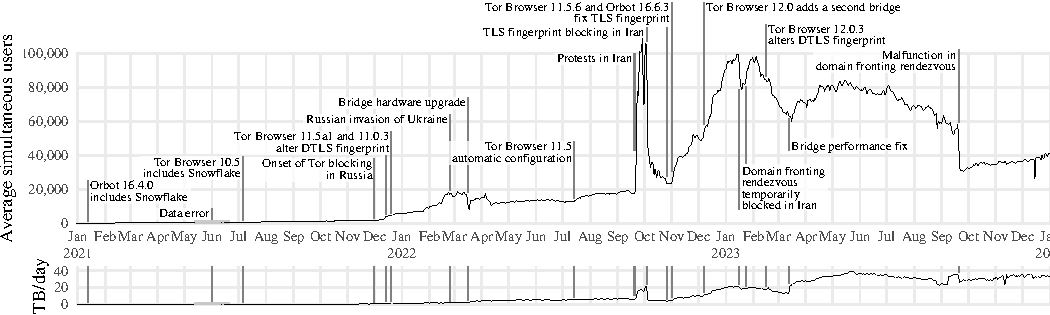
\includegraphics{figures/users/users-global}
\caption{
Estimated average simultaneous Snowflake users and bandwidth by day.
The values at the far left end of the graph,
in~early July~2021, are about~200 users
% > filter(filtered, abs(date - as.Date("2021-07-01")) < 3)
% # A tibble: 5 × 3
%   date       transport users
%   <date>     <chr>     <dbl>
% 1 2021-06-29 snowflake  278.
% 2 2021-06-30 snowflake  282.
% 3 2021-07-01 snowflake  262.
% 4 2021-07-02 snowflake  199.
% 5 2021-07-03 snowflake  197.
and 2.7~Mbit/s.
% > library("tidyverse")
% > WANTED_FINGERPRINTS <- c(
%     "7659DA0F96B156C322FBFF3ACCC9B9DC01C27C73" = "snowman",
%     "5481936581E23D2D178105D44DB6915AB06BFB7F" = "snowflake-01",
%     "91DA221A149007D0FD9E5515F5786C3DD07E4BB0" = "snowflake-02"
%   )
% > options(width = 200)
% > userstats <- read_csv("figures/users/userstats-bridge-transport-multi.csv") %>%
%     filter(fingerprint %in% names(WANTED_FINGERPRINTS)) %>%
%     mutate(users = users / (coverage / pmax(num_instances, coverage)))
% > bandwidth <- read_csv("figures/users/bandwidth-multi.csv") %>%
%     filter(fingerprint %in% names(WANTED_FINGERPRINTS)) %>%
%     filter(coverage > 0) %>%
%     mutate(bytes = bytes / (coverage / pmax(num_instances, coverage))) %>%
%     pivot_wider(id_cols = c(date, fingerprint), names_from = c(type), values_from = c(bytes)) %>%
%     mutate(
%       good_read = read - `dirreq-read`,
%       good_write = write - `dirreq-write`,
%       good_avg = (good_read + good_write) / 2,
%       good_avg_bps = good_avg*8/86400,
%     )
% > left_join(userstats, bandwidth, by = c("date", "fingerprint")) %>%
%     # Subtract out the pro-rated fraction of non-snowflake transports (basically negligible).
%     group_by(date, fingerprint) %>%
%     mutate(across(c(read, write, `dirreq-read`, `dirreq-write`, good_read, good_write, good_avg), ~ .x * users / sum(users))) %>%
%     ungroup() %>%
%     filter(transport == "snowflake") %>%
%     filter("2021-06-28" <= date & date < "2021-07-04") %>%
%     group_by(date) %>%
%     summarize(
%       date = last(date),
%       across(c(read, write, `dirreq-read`, `dirreq-write`, good_read, good_write, good_avg, good_avg_bps), sum, na.rm = TRUE)
%     ) %>%
%     mutate(
%       across(c(read, write, `dirreq-read`, `dirreq-write`, good_read, good_write, good_avg), scales::label_bytes(units = "auto_si", accuracy = 0.01)),
%       across(c(good_avg_bps), scales::label_number(scale_cut = scales::cut_si("bit"), accuracy = 0.01)),
%     ) %>%
%     arrange(date) %>% tail()
% # A tibble: 6 × 9
%   date       read     write    `dirreq-read` `dirreq-write` good_read good_write good_avg good_avg_bps
%   <date>     <chr>    <chr>    <chr>         <chr>          <chr>     <chr>      <chr>    <chr>
% 1 2021-06-28 43.69 GB 45.14 GB 414.49 MB     5.03 GB        43.28 GB  40.11 GB   41.69 GB 3.86 Mbit
% 2 2021-06-29 32.92 GB 34.41 GB 404.10 MB     4.92 GB        32.51 GB  29.49 GB   31.00 GB 2.87 Mbit
% 3 2021-06-30 32.20 GB 34.24 GB 419.36 MB     5.06 GB        31.79 GB  29.18 GB   30.48 GB 2.83 Mbit
% 4 2021-07-01 31.17 GB 32.60 GB 354.75 MB     4.25 GB        30.82 GB  28.35 GB   29.58 GB 2.74 Mbit
% 5 2021-07-02 27.72 GB 27.40 GB 178.13 MB     2.15 GB        27.54 GB  25.25 GB   26.40 GB 2.44 Mbit
% 6 2021-07-03 28.02 GB 27.92 GB 200.54 MB     2.45 GB        27.82 GB  25.47 GB   26.64 GB 2.47 Mbit
}
\label{fig:client-counts}
\end{figure*}

\section{Experience}
\label{sec:experience}

Snowflake has now been in operation for a few years.
In~lieu of a forward-looking evaluation,
here we take a look back
at the history of our deployment
and reflect on the experience.

\subsection{Client counts and bandwidth}
\label{sec:clients}

% Excerpts from https://gitlab.torproject.org/tpo/network-health/metrics/timeline:
% |2017-01-24|||snowflake|Tor Browser 7.0a1 released, including Snowflake for GNU/Linux only.|[blog post](https://blog.torproject.org/blog/tor-browser-70a1-released)||
% |2017-08-08|||snowflake|Tor Browser 7.5a4 released, including Snowflake for macOS.|[blog post](https://blog.torproject.org/blog/tor-browser-75a4-released) [issue](https://bugs.torproject.org/tpo/applications/tor-browser/22831)||
% |2018-03-26 20:43:42|||snowflake|Release of Tor Browser 8.0a5. Improves snowflake client performance.|[blog post](https://blog.torproject.org/tor-browser-80a5-released) [ticket](https://bugs.torproject.org/tpo/anti-censorship/pluggable-transports/snowflake/21312)||
% |2019-10-01|||snowflake|Release of Tor Browser 9.0a7, the first release that has Snowflake for Windows.|[blog post](https://blog.torproject.org/new-release-tor-browser-90a7) [ticket](https://bugs.torproject.org/tpo/anti-censorship/pluggable-transports/snowflake/25483)||
% |2020-05-22 19:51:29|||snowflake|Release of Tor Browser 9.5a13, the first release with Turbo Tunnel session persistence features for Snowflake. There is a spike in estimated users on 2020-05-21 and 2020-05-22, which appears to be an artifact.|[blog post](https://blog.torproject.org/new-release-tor-browser-95a13) [ticket](https://bugs.torproject.org/tpo/applications/tor-browser/34043) [users graph](https://metrics.torproject.org/userstats-bridge-transport.html?start=2020-03-01&end=2020-08-01&transport=snowflake)||
% |2020-06-02 18:09:48|||snowflake|Release of Tor Browser 10.0a1, the first release with Snowflake for Android.|[blog post](https://blog.torproject.org/new-release-tor-browser-100a1) [ticket](https://bugs.torproject.org/tpo/applications/tor-browser/30318)||
% |2020-06-25|2020-06-25||snowflake|One- or two-day spike in estimated Snowflake users. It resembles the spike that occurred around the time of the Turbo Tunnel release of Tor Browser 9.5a13 on 2020-05-22.|[users graph](https://metrics.torproject.org/userstats-bridge-transport.html?start=2020-03-01&end=2020-08-01&transport=snowflake)|X|
% |2020-08-19|||snowflake|Release of Tor Browser 10.0a5, which added added the ability to do NAT behavior discovery to the Snowflake client.|[blog post](https://blog.torproject.org/new-release-tor-browser-100a5/) [issue](https://bugs.torproject.org/tpo/applications/tor-browser-build/40016)||
% |2020-10-29|||snowflake|Release of Snowflake WebExtension 0.5.0, with a NAT type self-test.|[archive](https://archive.org/details/snowflake-webextension-0.5.0) [issue](https://bugs.torproject.org/tpo/anti-censorship/pluggable-transports/snowflake/40013)||
% |2020-11-17|||snowflake|Release of Snowflake WebExtension 0.5.2, with a fix to the NAT type self-test.|[archive](https://archive.org/details/snowflake-webextension-0.5.2) [merge request](https://gitlab.torproject.org/tpo/anti-censorship/pluggable-transports/snowflake-webext/-/merge_requests/9) [comment](https://bugs.torproject.org/tpo/anti-censorship/pluggable-transports/snowflake/40013#note_2716071)||
% |2021-01-12|||snowflake|Release of Orbot 16.4.0-RC-1-tor-0.4.4.6, first release with Snowflake client support.|[release](https://github.com/guardianproject/orbot/releases/tag/16.4.0-RC-1-tor-0.4.4.6)||
% |2021-02-23|||snowflake|Release of Orbot 16.4.1-BETA-2-tor.0.4.4.6, with experimental Snowflake proxy support.|[release](https://github.com/guardianproject/orbot/releases/tag/16.4.1-BETA-2-tor.0.4.4.6)||
% |2021-07-06 16:56:37|||snowflake|Release of Tor Browser 10.5, first stable release that includes Snowflake.|[blog post](https://blog.torproject.org/new-release-tor-browser-105)||
% |2021-12-01|ongoing|ru||Blocking of Tor directory authorities, relays, default obfs4 bridges, meek-azure, and Snowflake in some ISPs in Russia. There was a temporary cease of blocking for less than a day starting on 2021-12-08.|[NTC thread](https://ntc.party/t/ooni-reports-of-tor-blocking-in-certain-isps-since-2021-12-01/1477) [BBS thread](https://github.com/net4people/bbs/issues/97) [issue](https://bugs.torproject.org/tpo/community/support/40050) [blog post](https://blog.torproject.org/tor-censorship-in-russia/) [OONI report](https://ooni.org/post/2021-russia-blocks-tor/#blocking-of-the-tor-network)||
% |2021-12-14|||snowflake|Release of Tor Browser 11.5a1, with an altered DTLS fingerprint in Snowflake to counteract blocking in Russia.|[blog post](https://blog.torproject.org/new-release-tor-browser-115a1/) [issue](https://bugs.torproject.org/tpo/applications/tor-browser-build/40393) [NTC post](https://ntc.party/t/ooni-reports-of-tor-blocking-in-certain-isps-since-2021-12-01/1477/59)||
% |2021-12-20|||snowflake|Release of Tor Browser 11.0.3, with an altered DTLS fingerprint in Snowflake to counteract blocking in Russia.|[blog post](https://blog.torproject.org/new-release-tor-browser-1103/) [issue](https://bugs.torproject.org/tpo/applications/tor-browser-build/40393) [NTC post](https://ntc.party/t/ooni-reports-of-tor-blocking-in-certain-isps-since-2021-12-01/1477/59)||
% |2022-01-25 17:41:00|||snowflake|Switched the snowflake bridge to a temporary load-balanced staging server. Debugged connection problems until 2022-01-25 18:47:00.|[issue](https://bugs.torproject.org/tpo/tpa/team/40598#note_2772287) [comment](https://bugs.torproject.org/tpo/anti-censorship/pluggable-transports/snowflake/40095#note_2772325) [post](https://forum.torproject.net/t/tor-relays-how-to-reduce-tor-cpu-load-on-a-single-bridge/1483/16) [comment](https://github.com/net4people/bbs/issues/103#issuecomment-1033067920)||
% |2022-03-16 16:51:35|||snowflake|Moved Snowflake traffic to the interim bridge running instances flakey1–flakey8.|[comment](https://bugs.torproject.org/tpo/tpa/team/40664#note_2787624)||
% |2022-05-06 12:14:51|||snowflake|Upgraded the network uplink of the Snowflake bridge from 1 Gbps to 10 Gbps.|[issue](https://bugs.torproject.org/tpo/anti-censorship/pluggable-transports/snowflake/40138)||
% |2022-06-27|||snowflake|Deployed version 0.6.0 of the Snowflake WebExtension. The main feature added in this release was support for more than one bridge. It had a bug that caused it to stop reporting client IP addresses, which are used for metrics purposes by the bridge.|[archive](https://archive.org/details/snowflake-webextension-0.6.0) [merge request](https://gitlab.torproject.org/tpo/anti-censorship/pluggable-transports/snowflake-webext/-/merge_requests/29) [issue](https://bugs.torproject.org/tpo/anti-censorship/pluggable-transports/snowflake-webext/82)||
% |2022-07-14|||bridge|Release of Tor Browser 11.5, with a new feature of automatic censorship circumvention configuration.|[blog post](https://blog.torproject.org/new-release-tor-browser-115/)||
% |2022-09-21|ongoing|ir||Protests and daily Internet shutdowns in Iran.|[OONI report](https://ooni.org/post/2022-iran-blocks-social-media-mahsa-amini-protests/) [BBS thread](https://github.com/net4people/bbs/issues/125)||
% |2022-10-03 12:50:34|||snowflake|Deployment of Snowflake broker to reject proxies that do not support multiple bridges.|[issue](https://bugs.torproject.org/tpo/anti-censorship/pluggable-transports/snowflake/40193) [issue](https://bugs.torproject.org/tpo/anti-censorship/team/95)||
% |2022-10-04 17:15:00|||snowflake|Snowflake rendezvous blocked by TLS fingerprint in Iran.|[issue](https://bugs.torproject.org/tpo/anti-censorship/pluggable-transports/snowflake/40207) [BBS thread](https://github.com/net4people/bbs/issues/131)||
% |2022-10-12|||snowflake|Release of Tor Browser 11.5.4. Adds uTLS TLS camouflage support for Snowflake, making a manual configuration possible to circumvent recent TLS blocking in Iran.|[blog post](https://blog.torproject.org/new-release-tor-browser-1154/) [BBS comment](https://github.com/net4people/bbs/issues/131#issuecomment-1280391051)||
% |2022-10-17 15:52:00||ir|snowflake|Enabled uTLS for Snowflake in Iran in the Circumvention Settings API, using the `hellochrome_auto` fingerprint.|[comment](https://bugs.torproject.org/tpo/anti-censorship/team/96#note_2844378) [merge request](https://gitlab.torproject.org/tpo/anti-censorship/rdsys-admin/-/merge_requests/6)||
% |2022-10-20 15:16:00|||snowflake|Release of Orbot for Android 16.6.3-BETA-2-tor.0.4.7.10. Adds uTLS TLS camouflage support for Snowflake, making it possible to circumvent recent TLS blocking in Iran.|[release](https://github.com/guardianproject/orbot/releases/tag/16.6.3-BETA-2-tor.0.4.7.10) [announcement](https://github.com/net4people/bbs/issues/125#issuecomment-1285897627)||
% |2022-10-27|||snowflake|Release of Tor Browser 11.5.6. Fixes the problem that prevented Snowflake from working in 11.5.5, and enables uTLS TLS camouflage support by default for Snowflake.|[blog post](https://blog.torproject.org/new-release-tor-browser-1156/) [issue](https://bugs.torproject.org/tpo/applications/tor-browser-build/40665)||
% |2022-11-01||ir|snowflake|Orbot begins a gradual release rollout of version 16.6.3-RC-1-tor.0.4.7.10, which has TLS fingerprint changes to make Snowflake work in Iran again.|[release](https://github.com/guardianproject/orbot/releases/tag/16.6.3-RC-1-tor.0.4.7.10)||
% |2022-12-01|||snowflake|Release of Tor Browser 12.0a5, the first release to contain both the snowflake-01 and snowflake-02 bridges.|[issue](https://bugs.torproject.org/tpo/applications/tor-browser-build/40674) [announcement](https://lists.torproject.org/pipermail/tor-announce/2022-December/000256.html) [BBS comment](https://github.com/net4people/bbs/issues/152#issuecomment-1336220171)||
% |2022-12-07|||snowflake|Release of Tor Browser 12.0, the first stable release to contain both the snowflake-01 and snowflake-02 bridges.|[issue](https://bugs.torproject.org/tpo/applications/tor-browser-build/40674) [blog post](https://blog.torproject.org/new-release-tor-browser-120/) [BBS comment](https://github.com/net4people/bbs/issues/152#issuecomment-1342800169) [NTC comment](https://ntc.party/t/second-snowflake-bridge-available-for-testing/3445/2)||
% |2023-01-16|2023-01-24|ir|moat snowflake|The domain name cdn.sstatic.net, which is used by Snowflake and Moat, is blocked in some ISPs in Iran.|[comment](https://bugs.torproject.org/tpo/anti-censorship/team/115#note_2873040)||
% |2023-01-31|2023-02-01|ir|moat snowflake|The domain name cdn.sstatic.net, which is used by Snowflake and Moat, is again blocked in some ISPs in Iran.|[comment](https://bugs.torproject.org/tpo/anti-censorship/team/115#note_2876012)||
% |2023-02-08|2023-02-13|ir|moat snowflake|The domain name cdn.sstatic.net, which is used by Snowflake and Moat, is again blocked in some ISPs in Iran.|[comment](https://bugs.torproject.org/tpo/anti-censorship/team/115#note_2883298) [OONI chart](https://explorer.ooni.org/chart/mat?probe_cc=IR&since=2023-01-23&until=2023-03-01&time_grain=day&axis_x=measurement_start_day&test_name=web_connectivity&domain=cdn.sstatic.net)||
% |2023-02-15|||snowflake|Release of Tor Browser 12.0.3. Has a change to the Snowflake DTLS fingerprint (removes Hello Verify Request) to mitigate reported blocking in Russia.|[blog post](https://blog.torproject.org/new-release-tor-browser-1203/) [comment about Hello Verify Request](https://bugs.torproject.org/tpo/anti-censorship/censorship-analysis/40030#note_2823140) [Snowflake merge request](https://gitlab.torproject.org/tpo/anti-censorship/pluggable-transports/snowflake/-/merge_requests/134) [Tor Browser merge request](https://gitlab.torproject.org/tpo/applications/tor-browser-build/-/merge_requests/637)||
% |2023-02-19|2023-02-19|ir|moat snowflake|The domain name cdn.sstatic.net, which is used by Snowflake and Moat, is again blocked in some ISPs in Iran.|[comment](https://bugs.torproject.org/tpo/anti-censorship/team/115#note_2883298) [OONI chart](https://explorer.ooni.org/chart/mat?probe_cc=IR&since=2023-01-23&until=2023-03-01&time_grain=day&axis_x=measurement_start_day&test_name=web_connectivity&domain=cdn.sstatic.net)||
% |2023-02-22|2023-02-22|ir|moat snowflake|The domain name cdn.sstatic.net, which is used by Snowflake and Moat, is again blocked in some ISPs in Iran.|[comment](https://bugs.torproject.org/tpo/anti-censorship/team/115#note_2883298) [OONI chart](https://explorer.ooni.org/chart/mat?probe_cc=IR&since=2023-01-23&until=2023-03-01&time_grain=day&axis_x=measurement_start_day&test_name=web_connectivity&domain=cdn.sstatic.net)||
% |2023-03-13 19:46:07|||snowflake|Restarted snowflake-02 bridge for a bugfix.|[comment](https://bugs.torproject.org/tpo/anti-censorship/pluggable-transports/snowflake/40262#note_2886032) [issue](https://bugs.torproject.org/tpo/anti-censorship/pluggable-transports/snowflake/40260)||
% |2023-03-13 20:17:54|||snowflake|Restarted snowflake-01 bridge for a bugfix.|[comment](https://bugs.torproject.org/tpo/anti-censorship/pluggable-transports/snowflake/40262#note_2886041) [issue](https://bugs.torproject.org/tpo/anti-censorship/pluggable-transports/snowflake/40260)||
% |2023-03-15|||snowflake|Release of Orbot for Android v17 BETA 2. First release of Orbot to include the snowflake-02 bridge along with the existing snowflake-01. Has a change to the Snowflake DTLS fingerprint (removes Hello Verify Request) to mitigate reported blocking in Russia.|[release](https://github.com/guardianproject/orbot/releases/tag/17.0.0-BETA-2-tor.0.4.7.11) [Orbot commit adding snowflake-02](https://github.com/guardianproject/orbot/commit/c3f6ee18f17770a5904ad19c3cd24b9c8dcb3885) [IPtProxy commit upgrading Snowflake](https://github.com/tladesignz/IPtProxy/commit/5d0654a6a1439c05d3ee52b2b351b5df1ff3f6dc)||

Snowflake became available to end users gradually,
reflecting a long development process.
Development began in late 2015,
% 2015-10-01 initial commit in go-webrtc https://github.com/keroserene/go-webrtc/commit/a044c5aaa6cd8b7c66ca7863e35e1f1931677fc6
% 2015-12-22 initial commit in snowflake https://gitlab.torproject.org/tpo/anti-censorship/pluggable-transports/snowflake/-/commit/41c7613db85f6c1e8d13ea3639fb35d71f6ad942
and deployment in~2017,
but the system only really became usable in~2020.
It~began to attract large numbers of users
(enough to merit a censor's attention)
in~2022, following
network blocking events in Russia and Iran.

Snowflake shipped in the alpha release series of Tor Browser
before graduating to the stable series.
The first releases of Snowflake were
for GNU/Linux
in Tor Browser~7.0a1 on \mbox{2017-01-24}\,\urlfootnote{
% "Add snowflake pt to alpha linux builds"
https://bugs.torproject.org/tpo/applications/tor-browser/20735
% "First working bundles with Snowflake, for linux only" https://bugs.torproject.org/tpo/anti-censorship/pluggable-transports/snowflake/19001
}
and for macOS
in Tor Browser~7.5a4 on \mbox{2017-08-08}\,\urlfootnote{
% "Merge Snowflake for mac"
https://bugs.torproject.org/tpo/applications/tor-browser/22831
% "mac reproducible build" https://bugs.torproject.org/tpo/anti-censorship/pluggable-transports/snowflake/19001
% "[tbb-dev] Please check reproducibility of mac build with Snowflake (e084e83418)" https://lists.torproject.org/pipermail/tbb-dev/2017-July/000579.html
}.
But we hit a roadblock in attempting to prepare releases for other platforms:
the Chromium-derived WebRTC library we had used to that point
presented major difficulties
in Tor Browser's
cross-compiling, reproducible build environment.
What let us resume making progress was a switch to
Pion WebRTC~\cite{pion-webrtc} in~2019.
With it, we~were able to release
Snowflake for Windows
in Tor Browser~9.0a7 on \mbox{2019-10-01}\,\urlfootnote{
% "Windows reproducible build of snowflake"
https://bugs.torproject.org/tpo/anti-censorship/pluggable-transports/snowflake/25483
},
and for Android in
Tor Browser~10.0a1 on \mbox{2020-06-02}\,\urlfootnote{
% "Integrate snowflake into mobile Tor Browser alpha"
https://bugs.torproject.org/tpo/applications/tor-browser/30318
% "Android reproducible build of Snowflake" https://bugs.torproject.org/tpo/applications/tor-browser/28672
}.

While at this point Snowflake was available
on every platform supported by Tor Browser,
it was not yet comfortably usable.
Two important parts were missing:
no~NAT type matching (\autoref{sec:connection})
meant that a client could not always connect to its assigned proxy;
and a lack of persistent session state (\autoref{sec:data-transfer})
meant that even if a proxy connection was successful,
the client's session would end once that proxy disappeared.
For these reasons, by early 2020,
the average number of concurrent users
had not risen above~40.
% > library("tidyverse")
% > WANTED_FINGERPRINTS <- c(
%     "7659DA0F96B156C322FBFF3ACCC9B9DC01C27C73" = "snowman",
%     "5481936581E23D2D178105D44DB6915AB06BFB7F" = "snowflake-01",
%     "91DA221A149007D0FD9E5515F5786C3DD07E4BB0" = "snowflake-02"
%   )
% > userstats <- read_csv("figures/users/userstats-bridge-transport-multi.csv") %>%
%     filter(transport == "snowflake" & fingerprint %in% names(WANTED_FINGERPRINTS)) %>%
%     mutate(users = users / (coverage / pmax(num_instances, coverage))) %>%
%     group_by(date, transport) %>% summarize(users = sum(users, na.rm = TRUE), .groups = "drop")
%
% Ignoring two apparently anomalous spikes before 2021.
% One on 2020-05-21 and 2020-05-22 (the day of the Turbo Tunnel release):
% > filter(userstats, "2020-05-19" <= date & date <= "2020-05-24")
% # A tibble: 6 x 3
%   date       transport  users
%   <date>     <chr>      <dbl>
% 1 2020-05-19 snowflake   9.16
% 2 2020-05-20 snowflake  14.7
% 3 2020-05-21 snowflake 133.
% 4 2020-05-22 snowflake 388.
% 5 2020-05-23 snowflake   7.9
% 6 2020-05-24 snowflake  13.9
% One on 2020-06-25 and 2020-06-26 (not sure what this one is about):
% > filter(userstats, "2020-06-23" <= date & date <= "2020-06-28")
% # A tibble: 6 x 3
%   date       transport users
%   <date>     <chr>     <dbl>
% 1 2020-06-23 snowflake  17.0
% 2 2020-06-24 snowflake  20.2
% 3 2020-06-25 snowflake  71.7
% 4 2020-06-26 snowflake 211.
% 5 2020-06-27 snowflake  22.5
% 6 2020-06-28 snowflake  33.7
%
% > filtered <- filter(userstats, !(date %in% as.Date(c("2020-05-21", "2020-05-22", "2020-06-25", "2020-06-26"))))
% > filtered[which.max(filter(filtered, date < "2020-05-21")$users), ]
% # A tibble: 1 x 3
%   date       transport users
%   <date>     <chr>     <dbl>
% 1 2020-04-01 snowflake  34.0
The Turbo Tunnel session persistence feature
became available to users in Tor Browser~9.5a13
on \mbox{2020-05-22}.\urlfootnote{
% "Merge a turbotunnel branch"
https://bugs.torproject.org/tpo/anti-censorship/pluggable-transports/snowflake/33745
% "Update snowflake to persist sessions across proxies" https://bugs.torproject.org/tpo/applications/tor-browser/34043
}
The client part of NAT behavior detection
was released with Tor Browser~10.0a5 on \mbox{2020-08-19}\,\urlfootnote{
% "Use STUN to determine NAT behaviour of peers"
https://bugs.torproject.org/tpo/anti-censorship/pluggable-transports/snowflake/34129
% "Update snowflake version and prefs to do nat discovery at the client" https://bugs.torproject.org/tpo/applications/tor-browser-build/40016
},
and proxy support was added on \mbox{2020-11-17}\,\urlfootnote{
% "Have a remote probe service to test snowflake proxy NAT compatability"
https://bugs.torproject.org/tpo/anti-censorship/pluggable-transports/snowflake/40013
% "Wait for ice gathering to complete before probtest" https://gitlab.torproject.org/tpo/anti-censorship/pluggable-transports/snowflake-webext/-/merge_requests/9
% "after merging snowflake-webext!9 (merged), this is finally working" https://bugs.torproject.org/tpo/anti-censorship/pluggable-transports/snowflake/40013#note_2716071
% https://archive.org/details/snowflake-webextension-0.5.2
}.
With these changes, Snowflake became practical for daily browsing,
and the number of users began to grow into~2021.

This brings us to \autoref{fig:client-counts}, which
shows the Snowflake users and daily bandwidth since July 2021.
Be aware: the chart does not show a count of unique clients,
but rather the \emph{average number of concurrent clients} per day~\cite{tor-tr-2012-10-001}.
% "The result is an average number of concurrent users, estimated from data collected over a day. We can't say how many distinct users there are."
% https://metrics.torproject.org/reproducible-metrics.html#users
% $ grep '^2022-05-01.*,snowflake,' figures/users/userstats-bridge-transport-multi.csv
% 2022-05-01,5481936581E23D2D178105D44DB6915AB06BFB7F,snowflake,12235.62,100.00
For example, the value of 12,000 on \mbox{2022-05-01}
means that, on~average, 12,000 clients were using the service
at any point in time on that day.
The contribution of a client depends on how long it uses the system each day,
not how many temporary proxies it uses. The average concurrent client count is
estimated from the number of directory requests that are published in the descriptors
sent by Tor bridges to the bridge authority and archived by CollecTor.\urlfootnote{
https://metrics.torproject.org/collector.html\#type-extra-info
}
This method of estimating usage metrics was developed specifically to
preserve user anonymity. We discuss the techniques and challenges of
obtaining country-specific usage counts more in \autoref{sec:block} where we provide measurements
of Snowflake usage in response to censorship events.

Snowflake's growth began in earnest
when it became part of default installations.
Orbot, a mobile app that provides a VPN-like Tor proxy,
added a Snowflake client in version 16.4.0
on \mbox{2021-01-12}.\urlfootnote{
% 2021-01-12
https://github.com/guardianproject/orbot/releases/tag/16.4.0-RC-1-tor-0.4.4.6 2021-01-12
% https://github.com/guardianproject/orbot/blob/a69f39bb37469e65730d0751519848ec29001959/CHANGELOG#L788 /** 16.4.0-RC-1-tor-0.4.4.6 / 12 January 2021 **/
% "First version of Orbot with Snowflake, 16.4.0 on 2021-01-12?" https://lists.mayfirst.org/pipermail/guardian-dev/2023-July/005704.html
}
Snowflake graduated to Tor Browser's stable series
in Tor Browser~10.5
on \mbox{2021-07-06}\,\urlfootnote{
https://blog.torproject.org/new-release-tor-browser-105
},
becoming a third built-in circumvention option
alongside meek and obfs4.
% https://gitlab.torproject.org/tpo/applications/tor-browser-build/-/blob/tbb-10.5-build1/projects/tor-browser/Bundle-Data/PTConfigs/bridge_prefs.js
Being part of a stable release meant that it was
easily available to all Tor users,
not just a self-selected group of alpha testers.
The number of users steadily increased
over the next five months,
reaching almost~2,000 by December~2021.

A~network censorship event may have the effect
of either increasing or decreasing the number of users
of a circumvention system.
The user count decreases
when the system is not robust enough and falls to blocking;
but increases when it remains one
of a diminished number of ways to reach the outside world.
Two such censorship events,
one in Russia and one in Iran,
had the effect of increasing the number of Snowflake users
by multiples.

On \mbox{2021-12-01}, some ISPs in Russia
deployed measures to block
most forms of access to Tor,
including Snowflake~\cite{ooni-2021-russia-blocks-tor}.
The measures varied in their effectiveness;
in~the case of Snowflake,
blocking was triggered by a particular feature of the DTLS handshake
which we were able to mitigate in new releases within a few weeks.\urlfootnote{
% "Point to a forked version of pion/dtls with fingerprinting fix"
https://bugs.torproject.org/tpo/applications/tor-browser-build/40393
% "All right, finally managed to circumvent the censorship." https://bugs.torproject.org/tpo/anti-censorship/pluggable-transports/snowflake/40014#note_2765074
% https://blog.torproject.org/new-release-tor-browser-115a1/
% https://blog.torproject.org/new-release-tor-browser-1103/
}
Over the next two months the total number of Snowflake users quadrupled.
By~May 2022,
about 70\% of Snowflake users were in Russia.
% > library("tidyverse")
% > WANTED_FINGERPRINTS <- c(
%     "7659DA0F96B156C322FBFF3ACCC9B9DC01C27C73" = "snowman",
%     "5481936581E23D2D178105D44DB6915AB06BFB7F" = "snowflake-01",
%     "91DA221A149007D0FD9E5515F5786C3DD07E4BB0" = "snowflake-02"
%   )
% > userstats <- read_csv("figures/users/userstats-bridge-combined-multi.csv") %>%
%     filter(transport == "snowflake" & fingerprint %in% names(WANTED_FINGERPRINTS)) %>%
%     mutate(across(c(low, high), ~ .x / (coverage / pmax(num_instances, coverage)))) %>%
%     mutate(users = (low + high) / 2) %>%
%     # Combine the contributions of all bridges.
%     group_by(date, transport, country) %>% summarize(across(c(low, high, users), sum), .groups = "drop") %>%
%     # Apportion "??" to other countries (see figures/users/users-country.r).
%     group_by(date, transport) %>% mutate(across(c(low, high, users), ~ .x * sum(.x) / sum(ifelse(country == "??", 0, .x)))) %>% ungroup() %>% filter(country != "??")
% > userstats %>% filter(date == "2022-05-20") %>% arrange(desc(users)) %>%
%     mutate(percent = users / sum(users) * 100) %>% head()
% # A tibble: 6 x 7
%   date       transport country   low  high users percent
%   <date>     <chr>     <chr>   <dbl> <dbl> <dbl>   <dbl>
% 1 2022-05-20 snowflake ru      9311. 9311. 9311.   70.4
% 2 2022-05-20 snowflake us      1108. 1109. 1109.    8.38
% 3 2022-05-20 snowflake cn       533.  535.  534.    4.04
% 4 2022-05-20 snowflake de       256.  258.  257.    1.94
% 5 2022-05-20 snowflake by       200.  202.  201.    1.52
% 6 2022-05-20 snowflake gb       184.  186.  185.    1.40
The user count in Russia got an additional small boost,
visible in the graph,
starting on \mbox{2022-07-14},
when Tor Browser~11.5 added the Connection Assist feature,
which automatically enables circumvention options when needed.\urlfootnote{
https://blog.torproject.org/new-release-tor-browser-115/
% Graph showing boost going mostly to Russia: https://bugs.torproject.org/tpo/anti-censorship/pluggable-transports/snowflake-webext/82#note_2891387
}
We~will present more details of blocking actions in Russia
and their effect on usage in \autoref{sec:block-ru}.

% "Shutdowns, intensified blocking in Iran since 2022-09-21" https://github.com/net4people/bbs/issues/125
% "Need to increase number of tor instances on snowflake-01 bridge, increased usage since yesterday [2022-09-21]" https://lists.torproject.org/pipermail/anti-censorship-team/2022-September/000247.html
% "Graphs of user counts from Iran since the onset of shutdowns" https://forum.torproject.net/t/graphs-of-user-counts-from-iran-since-the-onset-of-shutdowns/4843
The next event to have a major effect on Snowflake usage
was the nationwide protests that started in Iran on \mbox{2022-09-16}.
The government imposed network shutdowns
and additional network blocking,
severe even by the standards of a country already notorious
for censorship~\cite{ooni-2022-iran-blocks-social-media-mahsa-amini-protests}.
Users turned to the few circumvention systems
that continued working in the face of the new restrictions,
one of which was Snowflake.
Adoption was rapid:
on~\mbox{2022-09-20}, Iran accounted for only~1\% of Snowflake users;
by~\mbox{2022-09-24} it was 67\%.
% > library("tidyverse")
% > WANTED_FINGERPRINTS <- c(
%     "7659DA0F96B156C322FBFF3ACCC9B9DC01C27C73" = "snowman",
%     "5481936581E23D2D178105D44DB6915AB06BFB7F" = "snowflake-01",
%     "91DA221A149007D0FD9E5515F5786C3DD07E4BB0" = "snowflake-02"
%   )
% > userstats <- read_csv("figures/users/userstats-bridge-combined-multi.csv") %>%
%     filter(transport == "snowflake" & fingerprint %in% names(WANTED_FINGERPRINTS)) %>%
%     mutate(across(c(low, high), ~ .x / (coverage / pmax(num_instances, coverage)))) %>%
%     mutate(users = (low + high) / 2) %>%
%     # Combine the contributions of all bridges.
%     group_by(date, transport, country) %>% summarize(across(c(low, high, users), sum), .groups = "drop") %>%
%     # Apportion "??" to other countries (see figures/users/users-country.r).
%     group_by(date, transport) %>% mutate(across(c(low, high, users), ~ .x * sum(.x) / sum(ifelse(country == "??", 0, .x)))) %>% ungroup() %>% filter(country != "??")
% > userstats %>% filter("2022-09-19" <= date & date <= "2022-09-25") %>%
%     group_by(date, transport) %>% mutate(percent = users / sum(users) * 100) %>% filter(country == "ir") %>% ungroup()
% # A tibble: 7 x 7
%   date       transport country    low   high  users percent
%   <date>     <chr>     <chr>    <dbl>  <dbl>  <dbl>   <dbl>
% 1 2022-09-19 snowflake ir        205.   207.   206.    1.20
% 2 2022-09-20 snowflake ir        228.   229.   228.    1.32
% 3 2022-09-21 snowflake ir       1024.  1025.  1024.    5.48
% 4 2022-09-22 snowflake ir      20920. 20909. 20914.   50.3
% 5 2022-09-23 snowflake ir      48467. 48427. 48447.   62.8
% 6 2022-09-24 snowflake ir      49130. 49083. 49107.   66.0
% 7 2022-09-25 snowflake ir      59517. 59470. 59493.   67.4
The influx of users had us scrambling for a few days
to implement performance improvements.
Two weeks later, on \mbox{2022-10-04},
usage dropped almost as quickly as it had risen---the
cause was the blocking of a TLS fingerprint
used by the Snowflake client.\urlfootnote{
% "Sudden reduction in snowflake-01 bridge bandwidth, 2022-10-04 17:15"
https://bugs.torproject.org/tpo/anti-censorship/pluggable-transports/snowflake/40207
}
After we released fixes for the TLS fingerprinting issue,
the user count began to recover going into 2023.
But in our haste to deploy optimizations in September,
we~had introduced a bug that harmed performance,
getting worse with more users\urlfootnote{
% "Weird KCP packets received by the client"
https://bugs.torproject.org/tpo/anti-censorship/pluggable-transports/snowflake/40260
},
which dragged the count down again,
until the bug was fixed in mid-March.
Umayya et~al.\ happened to do performance tests of Snowflake
during this time~\cite[\S 4.6]{Umayya2023a}---their results
bear out the lessened reliability of connections
before the performance bug was fixed\urlfootnote{
% "Deploy snowflake-server for QueuePacketConn buffer reuse fix (#40260)"
https://bugs.torproject.org/tpo/anti-censorship/pluggable-transports/snowflake/40262
}.
More details on blocking actions in Iran
will appear in \autoref{sec:block-ir}.

For most of this history,
we ran the backend bridge on a single server,
upgrading and optimizing it as needed.
But as the bridge reached its hardware capacity,
and performance improvements got harder to achieve,
we deployed a second bridge to share the load.
We discuss the challenges and design considerations of doing so in \autoref{sec:multi-bridge}.
The new bridge was made available in
Tor Browser~12.0 on \mbox{2022-12-07}.
By~July, it~supported about
18\% of users and
20\% of bandwidth.
% > library("tidyverse")
% > WANTED_FINGERPRINTS <- c(
%     "7659DA0F96B156C322FBFF3ACCC9B9DC01C27C73" = "snowman",
%     "5481936581E23D2D178105D44DB6915AB06BFB7F" = "snowflake-01",
%     "91DA221A149007D0FD9E5515F5786C3DD07E4BB0" = "snowflake-02"
%   )
% > userstats <- read_csv("figures/users/userstats-bridge-transport-multi.csv") %>%
%     filter(fingerprint %in% names(WANTED_FINGERPRINTS)) %>%
%     mutate(users = users / (coverage / pmax(num_instances, coverage)))
% > bandwidth <- read_csv("figures/users/bandwidth-multi.csv") %>%
%     filter(fingerprint %in% names(WANTED_FINGERPRINTS)) %>%
%     filter(coverage > 0) %>%
%     mutate(bytes = bytes / (coverage / pmax(num_instances, coverage))) %>%
%     pivot_wider(id_cols = c(date, fingerprint), names_from = c(type), values_from = c(bytes)) %>%
%     mutate(
%       good_read = read - `dirreq-read`,
%       good_write = write - `dirreq-write`,
%       good_avg = (good_read + good_write) / 2,
%     )
% > left_join(userstats, bandwidth, by = c("date", "fingerprint")) %>%
%     # Subtract out the pro-rated fraction of non-snowflake transports (basically negligible).
%     group_by(date, fingerprint) %>%
%     mutate(across(c(read, write, `dirreq-read`, `dirreq-write`, good_read, good_write, good_avg), ~ .x * users / sum(users))) %>%
%     ungroup() %>%
%     filter(transport == "snowflake") %>%
%     filter(date >= "2022-12-01") %>%
%     mutate(
%       year = lubridate::year(date),
%       month = lubridate::month(date),
%       instance = WANTED_FINGERPRINTS[fingerprint], fingerprint = NULL,
%     ) %>%
%     group_by(year, month, transport, instance) %>% summarize(users = sum(users), good_avg = sum(good_avg)) %>%
%     group_by(year, month, transport) %>%
%     mutate(
%       users_percent = 100 * users / sum(users, na.rm = TRUE),
%       bw_percent = 100 * good_avg / sum(good_avg, na.rm = TRUE),
%     ) %>% ungroup() %>% print(n = 30)
% # A tibble: 30 × 8
%     year month transport instance        users good_avg users_percent bw_percent
%    <dbl> <dbl> <chr>     <chr>           <dbl>    <dbl>         <dbl>      <dbl>
%  1  2022    12 snowflake snowflake-01 2043946.  4.40e14         98.0       96.3
%  2  2022    12 snowflake snowflake-02   42158.  1.67e13          2.02       3.66
%  3  2023     1 snowflake snowflake-01 2766748.  6.02e14         97.3       95.7
%  4  2023     1 snowflake snowflake-02   76198.  2.71e13          2.68       4.30
%  5  2023     2 snowflake snowflake-01 2286603.  4.72e14         96.3       93.8
%  6  2023     2 snowflake snowflake-02   88801.  3.10e13          3.74       6.16
%  7  2023     3 snowflake snowflake-01 1958580.  5.95e14         93.7       91.8
%  8  2023     3 snowflake snowflake-02  132598.  5.30e13          6.34       8.18
%  9  2023     4 snowflake snowflake-01 2044709.  7.97e14         89.4       86.2
% 10  2023     4 snowflake snowflake-02  242634.  1.27e14         10.6       13.8
% 11  2023     5 snowflake snowflake-01 2115663.  8.60e14         84.4       76.7
% 12  2023     5 snowflake snowflake-02  391264.  2.62e14         15.6       23.3
% 13  2023     6 snowflake snowflake-01 1889398.  8.21e14         81.6       76.8
% 14  2023     6 snowflake snowflake-02  425019.  2.48e14         18.4       23.2
% 15  2023     7 snowflake snowflake-01 1840693.  7.98e14         81.2       79.6
% 16  2023     7 snowflake snowflake-02  426490.  2.04e14         18.8       20.4
% 17  2023     8 snowflake snowflake-01 1718368.  7.55e14         83.9       84.0
% 18  2023     8 snowflake snowflake-02  328826.  1.44e14         16.1       16.0
% 19  2023     9 snowflake snowflake-01 1260765.  8.25e14         86.4       92.3
% 20  2023     9 snowflake snowflake-02  198159.  6.92e13         13.6        7.73
% 21  2023    10 snowflake snowflake-01  965871.  7.07e14         90.5       78.5
% 22  2023    10 snowflake snowflake-02  101105.  1.94e14          9.48      21.5
% 23  2023    11 snowflake snowflake-01  925517.  6.84e14         86.4       72.7
% 24  2023    11 snowflake snowflake-02  146157.  2.56e14         13.6       27.3
% 25  2023    12 snowflake snowflake-01 1000067.  7.51e14         85.2       73.7
% 26  2023    12 snowflake snowflake-02  173915.  2.68e14         14.8       26.3
% 27  2024     1 snowflake snowflake-01 1055248.  8.20e14         84.2       75.0
% 28  2024     1 snowflake snowflake-02  197708.  2.74e14         15.8       25.0
% 29  2024     2 snowflake snowflake-01   72876.  5.73e13         85.1       73.6
% 30  2024     2 snowflake snowflake-02   12764.  2.06e13         14.9       26.4

The drop in users by about half on \mbox{2023-09-20}
was not caused by censor action:
rather, it~was an unexpected change in the cloud
infrastructure we used for domain fronting rendezvous.
The front domain we had been using
changed its hosting to a different CDN,
which caused client rendezvous messages to fail to reach the broker.\urlfootnote{
% Problems with Snowflake since 2023-09-20: "broker failure Unexpected error, no answer."
https://forum.torproject.org/t/9346
% "[anti-censorship-team] Trying to understand multi-bridge dynamics post after Fastly/Cloudflare domain front change" https://lists.torproject.org/pipermail/anti-censorship-team/2023-September/000317.html
}
The user count began
to recover after we made releases
with alternative front domains.\urlfootnote{
% "Use foursquare as domain front for snowflake"
https://bugs.torproject.org/tpo/applications/tor-browser/42120
% "Randomly select front domain from comma-separated list" https://gitlab.torproject.org/tpo/anti-censorship/pluggable-transports/snowflake/-/merge_requests/182
% 2023-09-24 "New Alpha Release: Tor Browser 13.0a5 (Android, Windows, macOS, Linux)" https://blog.torproject.org/new-alpha-release-tor-browser-130a5/
% 2023-09-26 "New Release: Tor Browser 12.5.5" https://blog.torproject.org/new-release-tor-browser-1255/
}

As~of \mbox{2024-02-01},
Snowflake had transferred 13.9~PB of circumvention data.
% > library("tidyverse")
% > WANTED_FINGERPRINTS <- c(
%     "7659DA0F96B156C322FBFF3ACCC9B9DC01C27C73" = "snowman",
%     "5481936581E23D2D178105D44DB6915AB06BFB7F" = "snowflake-01",
%     "91DA221A149007D0FD9E5515F5786C3DD07E4BB0" = "snowflake-02"
%   )
% > options(width = 200)
% > userstats <- read_csv("figures/users/userstats-bridge-transport-multi.csv") %>%
%     filter(fingerprint %in% names(WANTED_FINGERPRINTS)) %>%
%     mutate(users = users / (coverage / pmax(num_instances, coverage)))
% > bandwidth <- read_csv("figures/users/bandwidth-multi.csv") %>%
%     filter(fingerprint %in% names(WANTED_FINGERPRINTS)) %>%
%     filter(coverage > 0) %>%
%     mutate(bytes = bytes / (coverage / pmax(num_instances, coverage))) %>%
%     pivot_wider(id_cols = c(date, fingerprint), names_from = c(type), values_from = c(bytes)) %>%
%     mutate(
%       good_read = read - `dirreq-read`,
%       good_write = write - `dirreq-write`,
%       good_avg = (good_read + good_write) / 2
%     )
% > left_join(userstats, bandwidth, by = c("date", "fingerprint")) %>%
%     # Subtract out the pro-rated fraction of non-snowflake transports (basically negligible).
%     group_by(date, fingerprint) %>%
%     mutate(across(c(read, write, `dirreq-read`, `dirreq-write`, good_read, good_write, good_avg), ~ .x * users / sum(users))) %>%
%     ungroup() %>%
%     filter(transport == "snowflake") %>%
%     filter(date < "2024-02-01") %>%
%     summarize(
%       date = last(date),
%       across(c(read, write, `dirreq-read`, `dirreq-write`, good_read, good_write, good_avg), sum, na.rm = TRUE)
%     ) %>%
%     mutate(across(c(read, write, `dirreq-read`, `dirreq-write`, good_read, good_write, good_avg), scales::label_bytes(units = "auto_si", accuracy = 0.01)))
% # A tibble: 1 × 8
%   date       read     write    `dirreq-read` `dirreq-write` good_read good_write good_avg
%   <date>     <chr>    <chr>    <chr>         <chr>          <chr>     <chr>      <chr>
% 1 2024-01-31 14.00 PB 14.03 PB 9.75 TB       181.10 TB      13.99 PB  13.85 PB   13.92 PB
We~are referring to goodput: Tor TLS traffic inside the tunnel,
ignoring WebRTC, WebSocket, and KCP/\allowbreak smux overhead.
At~that time, about 0.7\% of all Tor users
% It was a higher fraction before the addition of about 2 M users
% from Germany in June 2023:
% https://bugs.torproject.org/tpo/network-health/analysis/59
(24\%~of bridge users) used Snowflake to connect to Tor.
% > library("tidyverse")
% > WANTED_FINGERPRINTS <- c(
%     "7659DA0F96B156C322FBFF3ACCC9B9DC01C27C73" = "snowman",
%     "5481936581E23D2D178105D44DB6915AB06BFB7F" = "snowflake-01",
%     "91DA221A149007D0FD9E5515F5786C3DD07E4BB0" = "snowflake-02"
%   )
% > DATE_RANGE <- as.Date(c("2024-01-25", "2024-02-01"))
% > userstats <- bind_rows(
%     read_csv("figures/users/userstats-relay-country.csv", comment = "#") %>%
%       mutate(mode = "relay"),
%     read_csv("figures/users/userstats-bridge-transport.csv", comment = "#") %>%
%       filter(transport != "snowflake") %>%
%       mutate(mode = "bridge"),
%     # Use our own numbers for Snowflake users, rather than Tor Metrics'.
%     read_csv("figures/users/userstats-bridge-transport-multi.csv") %>%
%       filter(fingerprint %in% names(WANTED_FINGERPRINTS)) %>%
%       filter(transport == "snowflake") %>%
%       mutate(users = users / (coverage / pmax(num_instances, coverage))) %>%
%       group_by(date, transport) %>% summarize(users = sum(users, na.rm = TRUE), .groups = "drop") %>%
%       mutate(frac = 100, mode = "bridge")
%   ) %>%
%   filter(lubridate::`%within%`(date, do.call(lubridate::interval, as.list(DATE_RANGE)))) %>%
%     mutate(transport = if_else(mode == "bridge" & transport != "snowflake", "non-snowflake", transport)) %>%
%     group_by(mode, transport) %>% summarize(users = sum(users, na.rm = TRUE), .groups = "drop")
% > userstats %>% mutate(percent = 100 * users / sum(users))
% # A tibble: 3 × 4
%   mode   transport         users percent
%   <chr>  <chr>             <dbl>   <dbl>
% 1 bridge non-snowflake  1049214    2.14
% 2 bridge snowflake       335879.   0.684
% 3 relay  NA            47701971   97.2
% > userstats %>% filter(mode == "bridge") %>% mutate(percent = 100 * users / sum(users))
% # A tibble: 2 × 4
%   mode   transport        users percent
%   <chr>  <chr>            <dbl>   <dbl>
% 1 bridge non-snowflake 1049214     75.8
% 2 bridge snowflake      335879.    24.2

\subsection{Number and type of proxies}
\label{sec:proxies}

\begin{figure}
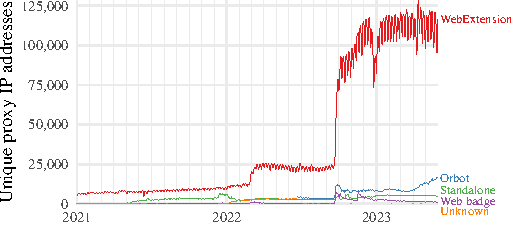
\includegraphics{figures/proxies/proxy-type}
\caption{
Unique proxy IP addresses per day,
by proxy type.
The two steps in the graph correspond
to the invasion of Ukraine by Russia in February~2022,
% 2022-02-25 https://twitter.com/torproject/status/1497276960556429324
% 2022-02-25 https://twitter.com/0xggus/status/1497224413829283877
and network restrictions in Iran beginning September~2022,
% 2022-09-24 https://twitter.com/torproject/status/1573670895696183303
% 2022-10-03 https://www.eff.org/deeplinks/2022/10/snowflake-makes-it-easy-anyone-fight-censorship
at which times there were campaigns
to encourage running Snowflake proxies.
Unknown proxy types (fewer than~50 instances) are not shown.
}
\label{fig:proxy-type}
% 2021-02-23 https://github.com/guardianproject/orbot/releases/tag/16.4.1-BETA-2-tor.0.4.4.6
% "experimental mode to enable running as a Snowflake proxy"
% 2021-07-14 https://github.com/tladesignz/IPtProxy/commit/228e9e61e285ee548a42d6bee487577e44630695
% IPtProxy 1.1.0 changes its proxy type from "standalone" to "iptproxy"
% 2021-12-20 https://github.com/guardianproject/orbot/releases/tag/16.5.2-RC-1-tor.0.4.6.8
% Orbot updates IPtProxy from 1.0.0 to 1.2.0 https://github.com/guardianproject/orbot/commit/57add48cd904afe94363219887cd142bb5cf6696
% 2022-01-03 https://github.com/guardianproject/orbot/releases/tag/16.5.2-RC-5-tor.0.4.6.9
% This is close to the date (2022-01-05) when there's sudden growth in "Unknown",
% which is probably Orbot self-reporting as "iptproxy" and the broker throwing away that label for being unrecognized.
% 2022-03-21 https://gitlab.torproject.org/tpo/anti-censorship/pluggable-transports/snowflake/-/merge_requests/82
% Broker starts to recognize "iptproxy" as a probe type, but not deployed yet.
% 2022-05-03 https://github.com/tladesignz/IPtProxy/commit/c6ba25ef6ce8449476f734c626eadffdf55d0519
% IPtProxy 1.6.0 adds 'ProxyType: "iptproxy"' (no effective change, had already been done in a patch).
% 2022-06-21 https://bugs.torproject.org/tpo/anti-censorship/pluggable-transports/snowflake/40151
% Broker deployment, broker starts recording "iptproxy" in descriptors.
% 2022-07-05 https://github.com/guardianproject/orbot/releases/tag/16.6.2-RC-1-tor.0.4.7.8
% Orbot 16.6.2 RC 1 upgrades to IPtProxy 1.6.0.
% 2022-08-02 https://github.com/guardianproject/orbot/releases/tag/17.0.0-ALPHA-1-tor.0.4.7.8
% "updated UI based on new design spec: https://github.com/guardianproject/orbot/blob/NEW_UX/docs/design-spec-kindness-mode.md"
% "improved support for Snowflake Proxying "kindness" / volunteer mode"
% 2023-01-13 https://github.com/guardianproject/orbot/releases/tag/17.0.0-BETA-1-tor.0.4.7.11
% "easy access to Snowflake proxy 'kindness' mode"
\end{figure}

Snowflake's effectiveness depends on its proxies,
of~which there are several types.
The primary type is the web browser extension,
% "Creating a Snowflake WebExtension addon" https://bugs.torproject.org/tpo/anti-censorship/pluggable-transports/snowflake/23888
which, once installed, works in the background
while the browser is running.
There is also a ``web badge'' version of the proxy that does not require installation.
It~uses the same JavaScript code as the extension, but runs in an ordinary web page.
Some people leave a browser tab idling on the web badge page,
rather than install a browser extension.
Apart from the web-based proxies,
we~provide a standalone, command-line proxy
that does not require a browser.
% "Golang implementation of standalone snowflake proxy" https://github.com/keroserene/snowflake/pull/41
This version is convenient to install on a rented VPS, for example.
Running a long-term proxy at a fixed IP address
is somewhat at odds with Snowflake's goal of proxy address diversity and agility,
but these standalone proxies are valuable because
they tend to have less restrictive NATs,
making them compatible with more clients.
Finally, Orbot, a mobile app for accessing Tor,
besides being able to \emph{use} Snowflake for circumvention,
can also \emph{provide} Snowflake proxy service to others,
a~feature called ``kindness mode.''
% Only so called in Orbot v17+, which should be current by the time the paper is submitted.
% As of 2024-02-09, according to Nathan in #guardianproject:matrix.org:
% Q: do you have a sense for what percentage of users are on the v16 track vs. v17?
% > A: 70% on v16, 30% on v17 out of 1.5 to 2M total active users

We coordinated with the Tor Project's network health team to collect privacy-preserving metrics at the broker
during the client and proxy polls of the Snowflake rendezvous.\urlfootnote{
https://bugs.torproject.org/tpo/network-health/metrics/collector/29461
}
The resulting metrics
are published at the end of every 24-hour collection period\urlfootnote{
https://metrics.torproject.org/collector.html\#snowflake-stats
}
in aggregate and we do not publish or store
client or proxy IP addresses. Metrics concerning client polls are rounded up to the nearest multiple
of~8 to prevent individual participation patterns from becoming visible in the aggregate counts.
The collected metrics allow us to determine daily unique proxy IP counts,
along with the associated country
codes, proxy types, NAT behavior types (restricted, unrestricted, or unknown), and how many times
a proxy was matched with a client.
\autoref{fig:proxy-type} shows the daily counts
of each proxy type.
Browser extension proxies predominate,
representing about 80\%
of 140,000 daily IP addresses.
% > library("tidyverse")
% > proxy_type <- read_csv("figures/proxies/proxy-type.csv", col_types = cols()) %>% filter("2024-01-01" <= date & date < "2024-02-01")
% > proxy_type %>% group_by(type) %>% summarize(unique_ips = sum(unique_ips / coverage)) %>% mutate(percent = 100 * unique_ips / sum(unique_ips)) %>% ungroup()
% # A tibble: 4 × 3
%   type       unique_ips percent
%   <chr>           <dbl>   <dbl>
% 1 badge          23016.   0.510
% 2 iptproxy      722234.  16.0
% 3 standalone    136748.   3.03
% 4 webext       3634973.  80.5
% > proxy_type %>% group_by(date) %>% summarize(unique_ips = sum(unique_ips / coverage)) %>% tail()
% # A tibble: 6 × 2
%   date       unique_ips
%   <date>          <dbl>
% 1 2024-01-26    147480.
% 2 2024-01-27    137645.
% 3 2024-01-28    139509.
% 4 2024-01-29    151370.
% 5 2024-01-30    152597.
% 6 2024-01-31    129535.
For comparison, there were about 1,900
of the more traditional style of Tor bridge at this time.
% https://metrics.torproject.org/networksize.csv?start=2024-01-01&end=2024-01-31
% date,relays,bridges
% 2024-01-29,7838,1950
% 2024-01-30,7851,1932
% 2024-01-31,7858,1931
The difference is attributable to the relative ease
of running a Snowflake proxy versus a Tor bridge---though
the comparison is not quite direct,
because Tor bridges have better defenses
against enumeration than do Snowflake proxies.
\todo{Find a place to talk about proxy geolocation and how proxies are measured.}

It~was not clear, at the outset,
that it would even be possible to attract
enough proxies to make Snowflake meaningfully blocking resistant
and support a reasonable number of users.
% "Start producing snowflakes" https://bugs.torproject.org/tpo/anti-censorship/pluggable-transports/snowflake/20813
Lowering the technical barriers to running a proxy was only part of~it;
getting there also took intentional advocacy and outreach.
In~the early days, circa~2017,
the only round-the-clock proxy support was
a few standalone proxies,
% 2018 "The three fallback proxy-go instances..." https://bugs.torproject.org/tpo/anti-censorship/pluggable-transports/snowflake/25688
run by us for the benefit of alpha tester clients.
The browser extension became available in mid-2019.\urlfootnote{
% |2019-06-26|||snowflake|Deployed version 0.0.1 of the Snowflake WebExtension for Firefox.|[comment](https://bugs.torproject.org/tpo/anti-censorship/pluggable-transports/snowflake/30931#note_2593598)||
https://bugs.torproject.org/tpo/anti-censorship/pluggable-transports/snowflake/30931\#note_2593598
}\textsuperscript,
% |2019-07-03|||snowflake|Deployed version 0.0.1 of the Snowflake WebExtension for Chrome.|[comment](https://bugs.torproject.org/tpo/anti-censorship/pluggable-transports/snowflake/30999#note_2593718)||
\urlfootnote{
https://bugs.torproject.org/tpo/anti-censorship/pluggable-transports/snowflake/30999\#note_2593718
}
In~the latter half of 2019,
% |2019-07-26|||flashproxy snowflake|Cupcake 2.0 is released, now working with Snowflake rather than flash proxy.|[Chrome Web Store page](https://chrome.google.com/webstore/detail/cupcake/dajjbehmbnbppjkcnpdkaniapgdppdnc)||
% Cupcake stopped working when we changed the proxy–broker protocol:
% |2019-11-13 16:47:02|||snowflake|Restarted the broker with a new proxy–broker protocol.|[comment](https://gitlab.torproject.org/tpo/anti-censorship/pluggable-transports/snowflake/-/issues/29207#note_2592849)||
additional proxy capacity came when Cupcake,
a~browser extension for flash proxy with an existing user base,
was repurposed for Snowflake.\urlfootnote{
% "Snowflake integration"
https://github.com/glamrock/cupcake/issues/24
% "Link Cupcake from snowflake.torproject.org"https://bugs.torproject.org/tpo/anti-censorship/pluggable-transports/snowflake/31497
}
Orbot's Snowflake proxy feature was added in version 16.4.1 in February~2021.\urlfootnote{
% 2021-02-23
https://github.com/guardianproject/orbot/releases/tag/16.4.1-BETA-2-tor.0.4.4.6
% https://github.com/guardianproject/orbot/releases/tag/16.4.1-RC-1-tor.0.4.4.6 2021-04-09
% https://github.com/guardianproject/orbot/blob/a69f39bb37469e65730d0751519848ec29001959/CHANGELOG#L714 /** 16.4.1-RC-1 / 9 April 2021 / c80f18ae2508b73fcbfd6e09b394a2a196de7459 **/
% https://lists.mayfirst.org/pipermail/guardian-dev/2023-July/005708.html
% 16.4.1-BETA-2-tor.0.4.4.6 was released and promoted first, and had a visible effect on proxy counts,
% though 16.4.1-RC-1-tor.0.4.4.6 was the "real" 16.4.1 release.
}
(In~\autoref{fig:proxy-type}, Orbot is counted among the standalone proxies
until January~2022, when it got its own proxy type designation.)
% See history in figures/proxies/proxy-type.r.

It~is worth reflecting
on the greater popularity of the browser extension
compared to the web badge.
The latter had been envisioned
as the primary source of proxies in flash proxy,
% By the end of its run, flash proxy had also gained
% https://www.bamsoftware.com/talks/ee380-flashproxy/index.html#s15
% browser extensions including Cupcake
% "Chrome browser add-on" [Cupcake for flash proxy] https://bugs.torproject.org/legacy/trac/7721
% "Tor Flashproxy Badge" [for Firefox] https://github.com/reezer/tor-flashproxy-badge/
% and a standalone proxy.
% "Node.js standalone flash proxy" https://bugs.torproject.org/legacy/trac/7944
the idea being that people's browsers
would automatically become proxies
while reading sites that had the flash proxy badge installed,
unless they checked an option to prevent~it.
We~decided, early on, that flash proxy's opt-out permission had been a mistake,
% Date: Tue, 6 Dec 2016 18:38:40 -0800
% From: David Fifield <dcf@torproject.org>
% To: Arlo Breault <arlo@torproject.org>
% Cc: Serene <serene@torproject.org>
% Subject: Re: Snowing
% Message-ID: <20161207023840.mli4cymr6s3aanpu@happy.bamsoftware.com>
%
% My original plan was to repurpose existing flash proxy badges as
% Snowflake badges. But, I am thinking more and more that Snowflake should
% use an opt-in model, rather than opt-out. The opt-out model of flash
% proxy always bothered me. I think there's a good chance it would cause
% trouble for us if Snowflake becomes popular. So I'd like to see
% Snowflake use opt-in badges (and Cupcake) only.
and that Snowflake would be opt-in.
In~order to run a proxy, a person must take a positive action
such as installing a browser extension
or activating a toggle on a web page.
% "Prepare a Snowflake 'options' page, like in flashproxy" https://github.com/keroserene/snowflake/issues/21
Our initial worry that this policy
would reduce the number of proxies turned out to be unfounded.
People find an informative, interactive proxy control panel more appealing
than a nondescript badge graphic,
and install the browser extension in greater numbers
than ever used the web badge in flash proxy.

\subsection{Proxy churn}
\label{sec:proxy-churn}

% https://bugs.torproject.org/tpo/anti-censorship/pluggable-transports/snowflake/34075
% https://gitlab.torproject.org/tpo/anti-censorship/pluggable-transports/snowflake/-/merge_requests/95

The size of the proxy pool is not the only measure of its quality.
Also important is its ``churn,'' the rate at which
it is replenished with fresh proxy IP addresses.
Churn determines how hard a censor would have to work
to keep a blocklist of proxy IP addresses up to date;
or alternatively,
how quickly a momentarily complete blocklist
would lose effectiveness.

We ran an experiment\urlfootnote{
https://bugs.torproject.org/tpo/anti-censorship/pluggable-transports/snowflake/34075
}
to measure churn.
Every hour, the broker logged a record of
the proxy IP addresses it had seen in the past hour.
To~avoid storing real proxy IP addresses,
each record was not a transparent list,
but a HyperLogLog++ sketch~\cite{Heule2013a},
a~probabilistic data structure for estimating
the number of distinct elements in a multiset.
We~additionally hashed proxy IP addresses with a secret string
before adding them to a sketch,
to prevent their recovery from our published data.
A~sketch supports two basic operations: count and merge.
Given a sketch~\(X\),
we may compute an approximate count \(|X|\)
of its unique elements,
and given two sketches \(X\) and~\(Y\),
we~may merge them into a new sketch
representing the union \(X \cup Y\).
The quantity we are interested in,
the size of the intersection of two sketches,
is~computed using the formula
\(|X| + |Y| - |X \cup Y|\).
Such a computation estimates
how many IP addresses are shared across
two samples of the proxy pool.

\begin{figure}
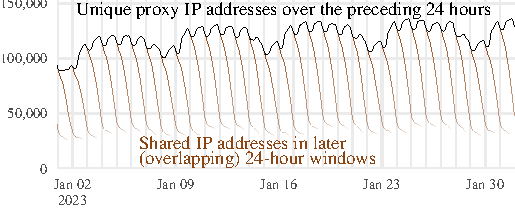
\includegraphics{figures/proxy-churn/proxy-count-decay}
\caption{
Proxy pool churn in January 2023.
The dark upper line shows the number
of unique proxy IP addresses in a 24-hour window
starting at the point indicated.
The lighter descending lines show
how many of the same IP addresses remain in the pool,
at 1-hour intervals up to 40 hours later.
It~takes about 20~hours for 50\% of the proxy pool to turn over.
}
\label{fig:proxy-count-decay}
\end{figure}

\autoref{fig:proxy-count-decay}
visualizes the results of the churn experiment.
We merged consecutive sketches over a 24-hour window
to serve as a reference,
then computed the size of its intersection
with other windows of the same size,
offset by \(+1, +2, \ldots, +40\) hours.
After 1~hour, the shifted window still has, on average,
97.3\% of addresses in common with the reference;
after 12~hours the fraction has fallen to 68.8\%;
by the time 24~hours have elapsed,
only 38.2\% of proxy IP addresses
are ones that had been seen in the previous day.
% > library("tidyverse")
% > options(width = 200)
% > DATE_RANGE <- as.Date(c("2023-01-01", "2023-02-01"))
% > read_csv("figures/proxy-churn/proxy-churn-windows.csv") %>%
%     filter(lubridate::`%within%`(reference_timestamp_end, do.call(lubridate::interval, as.list(DATE_RANGE)))) %>%
%     mutate(
%       sample_offset_hours = round(sample_timestamp_end_offset / 3600),
%       intersection_count = reference_count + sample_count - union_count
%     ) %>%
%     group_by(sample_offset_hours) %>%
%     summarize(
%       across(c(reference_count, sample_count, union_count, intersection_count), mean),
%       intersection_percent = 100 * intersection_count / reference_count,
%       .groups = "drop"
%     ) %>%
%     filter(sample_offset_hours %in% c(0, 1, 2, 3, 4, 8, 12, 18, 24, 36, 40))
% # A tibble: 11 x 6
%    sample_offset_hours reference_count sample_count union_count intersection_count intersection_percent
%                  <dbl>           <dbl>        <dbl>       <dbl>              <dbl>                <dbl>
%  1                   0         119654.      119654.     119654.            119654.                100
%  2                   1         119654.      119704.     122907.            116450.                 97.3
%  3                   2         119654.      119754.     126142.            113266.                 94.7
%  4                   3         119654.      119804.     129359.            110099.                 92.0
%  5                   4         119654.      119854.     132529.            106980.                 89.4
%  6                   8         119654.      120060.     145141.             94572.                 79.0
%  7                  12         119654.      120292.     157684.             82262.                 68.8
%  8                  18         119654.      120649.     176400.             63903.                 53.4
%  9                  24         119654.      120970.     194892.             45732.                 38.2
% 10                  36         119654.      121500.     206542.             34612.                 28.9
% 11                  40         119654.      121639.     208269.             33024.                 27.6

\subsection{Multiple bridges}
\label{sec:multi-bridge}

% "Prepare all pieces of the snowflake pipeline for a second snowflake bridge" https://bugs.torproject.org/tpo/anti-censorship/pluggable-transports/snowflake/28651
% "Distributed Snowflake Server Support" https://bugs.torproject.org/tpo/anti-censorship/pluggable-transports/snowflake/40129
% Ancient history from flash proxy: "allow the client to pick a specific relay for its registration" https://bugs.torproject.org/legacy/trac/10196

In the abstract model of \autoref{fig:architecture}, the bridge
is a single, centralized entity.
It~\emph{can} be centralized
because it is never accessed directly,
but only via temporary proxies.
Unlike more traditional static proxy systems,
Snowflake does not benefit, in terms of blocking resistance,
from having multiple bridges.
For scalability reasons, though,
it~is useful for ``the'' bridge to be realized as
multiple servers, each handling a fraction of client traffic.

Our deployment now uses two bridges.
Generalizing from one bridge to two
required changes to the messages exchanged between
clients, proxies, and the broker.
Unfortunately, the fact of multiple bridges
cannot be made fully transparent to clients,
for technical reasons related to Tor.
In~our design, the client informs the broker
of what bridge it wants to use,
the broker conveys the choice to the proxy,
and the proxy connects to the client's chosen bridge.
This is in contrast to other imaginable designs
where the choice of bridge is made
by the broker or the proxy.
We~will discuss design considerations and tradeoffs.

One minor difficulty is distributing the Turbo Tunnel layer.
Recall from \autoref{sec:data-transfer} that Snowflake
has the notion of an end-to-end session
between a client and the bridge,
independent of temporary proxy connections that carry~it.
This is made possible by extensive state stored at the bridge:
a~table of clients, reassembly buffers,
transmission queues, timers, and so~on.
% `type KCP` https://github.com/xtaci/kcp-go/blob/03b584b84eddd95cc03dbff65fc9cc5cbdf80c6b/kcp.go#L132
% `type UDPSession` https://github.com/xtaci/kcp-go/blob/03b584b84eddd95cc03dbff65fc9cc5cbdf80c6b/sess.go#L61
While it is certainly possible to instantiate one such
bundle of state variables per bridge,
a~session begun in one instance must remain with that instance---no other
has the context necessary to make the packets
of the session meaningful.
This difficulty might be resolved by hashing
the client's session identifier string to index
a consistent bridge per session,
as~long as the set of bridges does not change too frequently.

There is another difficulty that is harder to work around.
A~Tor bridge is identified
by a long-term identity public key.
If,~on connecting to a bridge,
the client finds that the bridge's identity is not the expected one,
the client will terminate the connection~\cite[\S 4.2]{tor-spec}.
% "As soon as it gets the CERTS cell, the initiator knows whether the responder is correctly authenticated." https://gitlab.torproject.org/tpo/core/torspec/-/blob/33308845cec54bfc0096b8ea0339a8ff183aa1b1/tor-spec.txt#L640
% connection_or_client_learned_peer_id https://gitlab.torproject.org/tpo/core/tor/-/blob/tor-0.4.7.13/src/core/or/connection_or.c#L1897
% [warn] Tried connecting to router at 192.0.2.3:80 ID=<none> RSA_ID=2B280B23E1107BB62ABFC40DDCC8824814F80A71, but RSA + ed25519 identity keys were not as expected: wanted 1111111111111111111111111111111111111111 + no ed25519 key but got 2B280B23E1107BB62ABFC40DDCC8824814F80A72 + 1zOHpg+FxqQfi/6jDLtCpHHqBTH8gjYmCKXkus1D5Ko.
% [warn] Problem bootstrapping. Stuck at 14% (handshake): Handshaking with a relay. (Unexpected identity in router certificate; IDENTITY; count 1; recommendation warn; host 1111111111111111111111111111111111111111 at 192.0.2.3:80)
The Tor client can configure at most one identity per bridge;
there is no way to indicate (with a certificate, for example)
that multiple identities should be considered equivalent.
This constraint leaves two options:
either all Snowflake bridges must share the same cryptographic identity,
or~else it must be the client that makes the choice of what bridge to use.
While the former option is possible to do
(by~synchronizing identity keys across servers),
every added bridge would increase the risk of compromising
the all-important identity keys.
Our vision was that different bridge sites
would run in different locations
with their own management teams,
and that any compromise of a bridge site
should affect that site only.

These considerations led us to a multi-bridge design
in which clients have awareness of (at~least a subset~of) all bridges,
and it is the client that chooses which bridge will be used
for a particular session.\urlfootnote{
https://bugs.torproject.org/tpo/anti-censorship/pluggable-transports/snowflake/28651\#note_2786323
}
The client includes a bridge identity string
in its rendezvous message to the broker (\autoref{sec:rendezvous});
then the broker maps the identity to the WebSocket URL
of the corresponding bridge,
and conveys that URL to the proxy
that's chosen to serve the client.
We~rely on clients choosing uniformly
to equalize load across bridges.
A~consequence is that
every bridge must meet a minimum performance standard:
we cannot, say,
centrally assign 20\% of clients to one and 80\% to another
according to their relative capacity.\todo{
Think about this more: snowflake-02
in fact has a consistent 15\% of users and 25\% of bandwidth.
}
Another drawback is that there is currently no way to instruct Tor
to connect to only one of the bridges it knows about
(short of rewriting the configuration file):
% "Let bridge users choose to only reach their first working bridge" https://bugs.torproject.org/tpo/core/tor/40578
if~two bridges are configured, Tor starts two sessions through Snowflake,
each doing its own rendezvous,
which is wasteful and makes for a more conspicuous network fingerprint.
Still, this is the best solution we have found, given the constraints.
A~deployment not based on Tor
would have more flexibility.

A~client-chooses design risks
misuse by clients, if~not handled carefully.
Clients should only be able to select from
a limited set of known bridges,
not cause proxies to connect to arbitrary destinations---otherwise
the tens of thousands of Snowflake proxies might be weaponized
to attack third parties.
% "Clients cannot cause a proxy to attack or even connect to an arbitrary web site or relay..." https://forum.torproject.net/t/anyone-experiencing-problems-with-snowflake-proxy/6938/15
% An alternative vision: "(More) Distributed servers" https://bugs.torproject.org/tpo/anti-censorship/pluggable-transports/snowflake/40248
% Flash proxy: "Remove 'facilitator', 'client', 'relay' query string parameters. ... These could be used to send unsolicited WebSocket connection attempts." https://gitlab.torproject.org/tpo/anti-censorship/pluggable-transports/flashproxy/-/compare/7c7acc14638a3e9346c99defa6d4dd80b4f437aa...d518f2615d977475dabaf4a46fbbe83c5a52801c
The client's bridge selection
in its rendezvous message is represented
not as an IP address or hostname,
but as a hash of the bridge's public identity key.
The broker maps the identity to a WebSocket URL
by consulting its own local database of known bridges,
and rejects rendezvous messages that refer to an unknown bridge.
% https://gitlab.torproject.org/tpo/anti-censorship/pluggable-transports/snowflake/-/blob/8e5ea8261110e97a8df56cfc9c83028081d902fb/broker/ipc.go#L187
After the broker tells the proxy what WebSocket URL to connect~to,
% https://gitlab.torproject.org/tpo/anti-censorship/pluggable-transports/snowflake/-/blob/8e5ea8261110e97a8df56cfc9c83028081d902fb/broker/ipc.go#L144
the proxy does its own check,
verifying that the hostname in the URL is a subdomain of
a known suffix reserved for Snowflake bridges.
So~there are two independent safeguards against misuse.

% \subsection{SQL injection attempts at broker}
% \url{https://bugs.torproject.org/tpo/anti-censorship/pluggable-transports/snowflake/40089}
% Actually tailored to the broker protocol, not a generic attack tool.

\section{Notable blocking attempts}
\label{sec:block}

In~\autoref{sec:clients} we saw how Snowflake's user counts
have at times been affected by the blocking actions of censors.
Now we take a closer look at selected censorship events.
The effect of censorship has usually been to increase, rather than decrease,
the number of Snowflake users.
This is no paradox:
as~censorship intensifies,
users are displaced from less resilient
to more resilient systems.
Snowflake's blocking resistance has not in every case been a success,
though, and here we also reflect on missteps
and persistent challenges.
The examples are taken from
Russia, Iran, China, and Turkmenistan,
and are selected for being significant and instructive.
Common lessons are that communication
with affected users is invaluable in quickly understanding and reacting to blocking;
and that blocking resistance is relative to a given censor,
because every censor's cost calculus is different.

Snowflake is blockable by a censor that is willing to block WebRTC.
We~would not argue otherwise.
Indeed, we~believe this is how a circumvention system
should be presented:
not by arguing its unblockability in absolute terms,
but by laying out
what actions by a censor would suffice to block~it---or~more
to the point,
\emph{what sacrifices a censor would have to make}
in order to block~it.
Advancing the state of the art of censorship circumvention
consists in pushing blocking
beyond the capabilities of more and more censors.

Tor bridges report aggregate binned counts by country code of connected unique IP addresses per day in the
descriptors uploaded to the bridge authority. We use the Tor Metrics method of
combining the distribution of counts by country code with the number of directory requests to obtain
an estimate of the average number of concurrent clients per day for each location~\cite{tor-tr-2012-10-001}. The mapping of IP
addresses to country codes is not without flaws. During the time of the measurements shown here, Tor uses
the IPFire location database.\urlfootnote{
https://www.ipfire.org/projects/location/
}
There is at least one instance where we were able to detect geolocation inaccuracies after noting
a significant drop in Snowflake users thought to be located in the US that correlated directly with
a blocking event in Iran.\urlfootnote{
https://bugs.torproject.org/tpo/anti-censorship/pluggable-transports/snowflake/40207\#note_2844116
}

\subsection{Blocking in Russia}
\label{sec:block-ru}

\begin{figure}
% Make the float take up an entire column.
% The \vphantom rule and \smash'ed minipage are because a plain minipage
% would count the depth of the descenders of the final line of text.
% See the TeXbook chapter 18, page 178.
% The output would otherwise look right, but yield a warning: Float too large for page by 2.18pt.
\vphantom{\rule{0pt}{\textheight}}\smash{%
\begin{minipage}[b][\textheight][b]{\linewidth}
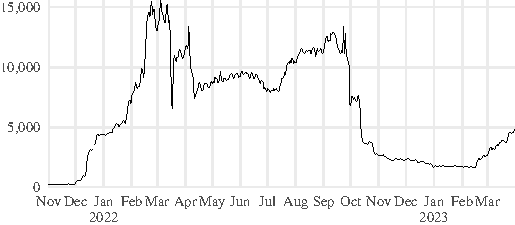
\includegraphics{figures/users/users-ru}
\caption{
Snowflake users in Russia (average concurrent).
Events discussed in the text are marked.
The attempted blocking of Tor-related transports in December~2021
led to Snowflake's first surge in usage.
The decrease in September--October~2022
coincided with an even larger influx from Iran.
\label{fig:client-counts-ru}
}
\vfill
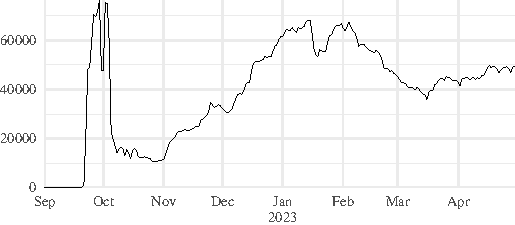
\includegraphics{figures/users/users-ir}
\caption{
Snowflake users in Iran.
Heightened censorship beginning in September 2022
caused Iran to become the single biggest source of Snowflake users.
The drop in October 2022
was the result of TLS fingerprint blocking,
which interfered with rendezvous
and took some time to mitigate.
\label{fig:client-counts-ir}
}
\vfill
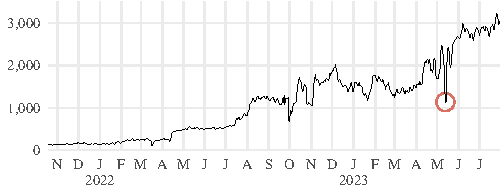
\includegraphics{figures/users/users-cn}
\caption{
Snowflake users in China.
Though no sustained blocking is evident,
disruption of domain fronting rendezvous
for three days in May 2023 briefly
depressed user numbers.
\label{fig:client-counts-cn}
}
\vfill
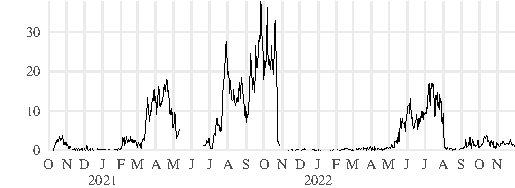
\includegraphics{figures/users/users-tm}
\caption{
Snowflake users in Turkmenistan.
This graph shows a different range of dates than the other three.
Though there have never been many Snowflake users in Turkmenistan,
blocking events are evident on
% > library("tidyverse")
% > WANTED_FINGERPRINTS <- c(
%     "7659DA0F96B156C322FBFF3ACCC9B9DC01C27C73" = "snowman",
%     "5481936581E23D2D178105D44DB6915AB06BFB7F" = "snowflake-01",
%     "91DA221A149007D0FD9E5515F5786C3DD07E4BB0" = "snowflake-02"
%   )
% > userstats <- read_csv("figures/users/userstats-bridge-combined-multi.csv") %>%
%     filter(transport == "snowflake" & fingerprint %in% names(WANTED_FINGERPRINTS)) %>%
%     mutate(across(c(low, high), ~ .x / (coverage / pmax(num_instances, coverage)))) %>%
%     mutate(users = (low + high) / 2) %>%
%     # Combine the contributions of all bridges.
%     group_by(date, transport, country) %>% summarize(across(c(low, high, users), sum), .groups = "drop") %>%
%     # Apportion "??" to other countries (see figures/users/users-country.r).
%     group_by(date, transport) %>% mutate(across(c(low, high, users), ~ .x * sum(.x) / sum(ifelse(country == "??", 0, .x)))) %>% ungroup() %>% filter(country != "??") %>%
%     filter(country == "tm")
% > userstats %>% filter("2021-10-20" <= date & date <= "2021-10-28")
% > userstats %>% filter("2022-07-30" <= date & date <= "2022-08-07")
% # A tibble: 9 × 6
%   date       transport country   low  high users
%   <date>     <chr>     <chr>   <dbl> <dbl> <dbl>
% 1 2021-10-20 snowflake tm      33.0  33.1  33.0
% 2 2021-10-21 snowflake tm      27.3  27.8  27.5
% 3 2021-10-22 snowflake tm      23.1  23.6  23.4
% 4 2021-10-23 snowflake tm      18.9  19.5  19.2
% 5 2021-10-24 snowflake tm       5.56  6.19  5.87
% 6 2021-10-25 snowflake tm       1.63  2.23  1.93
% 7 2021-10-26 snowflake tm       2.12  2.64  2.38
% 8 2021-10-27 snowflake tm       1.29  1.40  1.35
% 9 2021-10-28 snowflake tm       1.05  1.72  1.39
% # A tibble: 9 × 6
%   date       transport country   low   high users
%   <date>     <chr>     <chr>   <dbl>  <dbl> <dbl>
% 1 2022-07-30 snowflake tm       6.29  7.92  7.11
% 2 2022-07-31 snowflake tm       5.66  7.76  6.71
% 3 2022-08-01 snowflake tm       8.43 10.6   9.51
% 4 2022-08-02 snowflake tm       3.03  5.25  4.14
% 5 2022-08-03 snowflake tm       0     1.47  0.735
% 6 2022-08-04 snowflake tm       0     1.24  0.618
% 7 2022-08-05 snowflake tm       0     1.32  0.659
% 8 2022-08-06 snowflake tm       0     0.619 0.310
% 9 2022-08-07 snowflake tm       0     0.771 0.386
\mbox{2021-10-24} and \mbox{2022-08-03}.
% \label is inside \caption so that the baseline of the last line
% of the caption aligns with the baseline of the other column.
% https://tex.stackexchange.com/a/298714
\label{fig:client-counts-tm}
}
\end{minipage}}
\end{figure}

% "[Russia] Some ISPs are blocking Tor" https://bugs.torproject.org/tpo/community/support/40050
% "OONI reports of Tor blocking in certain ISPs since 2021-12-01" https://ntc.party/t/ooni-reports-of-tor-blocking-in-certain-isps-since-2021-12-01/1477
% "Responding to Tor censorship in Russia" https://blog.torproject.org/tor-censorship-in-russia/
% "OONI shows blocking of Snowflake in select ISPs in Russia since 2023-02" https://ntc.party/t/ooni-shows-blocking-of-snowflake-in-select-isps-in-russia-since-2023-02

Snowflake, along with other common ways of accessing Tor,
was blocked in a subset of ISPs in Russia
% https://ntc.party/t/ooni-reports-of-tor-blocking-in-certain-isps-since-2021-12-01/1477/95
% "Tor filtering is done using government black box called TSPU.
% Not all providers have them. Tor is not blocked if TSPU is not present.
% According to tor metrics graph directly connecting users decreased only by 1/3.
% This indicates TSPU is not everywhere."
on \mbox{2021-12-01}~\cite{ooni-2021-russia-blocks-tor}.
The event was evidently coordinated and targeted,
as~it happened suddenly and affected many Tor-related protocols at once.
Besides Snowflake,
a~portion of Tor relays and bridges,
as~well as some servers of
the circumvention transports meek and obfs4,
were blocked, at~least temporarily.
The blocking campaign was
less than totally successful---one
of its effects was to substantially increase the number
of users accessing Tor via circumvention transports,
Snowflake among them.
% "A zoom on just the bridge transports" https://bugs.torproject.org/tpo/community/support/40050#note_2796770
% That pluggable transports could not compensate fully
% for the loss of relay users points to a usability gap.

We~benefited from established relationships
with developers and users in Russia,
one of whom, through manual testing,
found what traffic feature was being used to distinguish Snowflake.
It~was DTLS fingerprinting,
of~the kind cautioned about in \autoref{sec:fingerprinting}.\urlfootnote{
% "Russian DPI check supported_groups extension in ServerHello payload (byte 0x5a in udp packet)."
https://bugs.torproject.org/tpo/anti-censorship/pluggable-transports/snowflake/40014\#note_2765074
}
Specifically, it~was the presence of a
\mbox{supported\_groups} extension in the DTLS Server Hello message produced by Pion.
The extension being present in Server Hello was a bug\urlfootnote{
% "Server Hello should not contain supported_groups extension (extension.SupportedEllipticCurves)"
https://github.com/pion/dtls/issues/409
}---but
one that afforded the censor a feature
to distinguish DTLS connections with a Pion implementation in the server role
from other forms of DTLS.
The process of finding the flaw, fixing it,
and shipping new releases of Tor Browser took a few weeks\urlfootnote{
% "Point to a forked version of pion/dtls with fingerprinting fix"
https://gitlab.torproject.org/tpo/applications/tor-browser-build/-/merge_requests/375
% 2021-12-14 https://blog.torproject.org/new-release-tor-browser-115a1/
% 2021-12-20 https://blog.torproject.org/new-release-tor-browser-1103/
},
after which the user count rose quickly:
from the beginning to the end of December~2021,
the number of users in Russia grew from about 400 to over 4,000
% > library("tidyverse")
% > WANTED_FINGERPRINTS <- c(
%     "7659DA0F96B156C322FBFF3ACCC9B9DC01C27C73" = "snowman",
%     "5481936581E23D2D178105D44DB6915AB06BFB7F" = "snowflake-01",
%     "91DA221A149007D0FD9E5515F5786C3DD07E4BB0" = "snowflake-02"
%   )
% > userstats <- read_csv("figures/users/userstats-bridge-combined-multi.csv") %>%
%     filter(transport == "snowflake" & fingerprint %in% names(WANTED_FINGERPRINTS)) %>%
%     mutate(across(c(low, high), ~ .x / (coverage / pmax(num_instances, coverage)))) %>%
%     mutate(users = (low + high) / 2) %>%
%     # Combine the contributions of all bridges.
%     group_by(date, transport, country) %>% summarize(across(c(low, high, users), sum), .groups = "drop") %>%
%     # Apportion "??" to other countries (see figures/users/users-country.r).
%     group_by(date, transport) %>% mutate(across(c(low, high, users), ~ .x * sum(.x) / sum(ifelse(country == "??", 0, .x)))) %>% ungroup() %>% filter(country != "??")
% > userstats %>% filter(date %in% as.Date(c("2021-12-01", "2022-01-01"))) %>% filter(country == "ru")
% # A tibble: 2 x 6
%   date       transport country   low  high users
%   <date>     <chr>     <chr>   <dbl> <dbl> <dbl>
% 1 2021-12-01 snowflake ru       381.  381.  381.
% 2 2022-01-01 snowflake ru      4381. 4380. 4380.
(\autoref{fig:client-counts-ru}).
Snowflake was to become a significant tool
amid the general intensification of censorship in Russia
following the invasion of Ukraine in February~2022.

The Server Hello \mbox{supported\_groups} distinguisher
had been
discovered and documented by MacMillan et~al.~\cite[\S 3]{arxiv.2008.03254}
already in~2020.
We~might have avoided this blocking event by proactively fixing
the known distinguisher---but
it was not necessarily the wrong call not to have done~so.
There is always more to do than time to do~it;
one must consider the opportunity cost
of preempting specific blocking that may not come to pass.
In~this case, a~reactive approach by us was enough:
the loss was minor, and we were able to patch the problem quickly.
Even in ISPs where the blocking rule was present,
it~did not block 100\% of Snowflake connections,
because of the how it targeted a quirk in Pion,
and only in Server Hello.
When the DTLS server role in the WebRTC data channel
was played by a non-Pion peer,
such as a web browser proxy,
the feature was not present.
% The Snowflake client would retry its rendezvous repeatedly,
% until hitting on a proxy that worked.

% "IRC Tip about Signature used to block Snowflake in Russia, 2022-May-16" https://bugs.torproject.org/tpo/anti-censorship/censorship-analysis/40030
% "Snowflake blocked by ClientHello [RU]" https://bugs.torproject.org/tpo/anti-censorship/pluggable-transports/snowflake/40140
% "A new Snowflake blocking rule (offset of supported_groups in DTLS Client Hello)" https://ntc.party/t/a-new-snowflake-blocking-rule-offset-of-supported-groups-in-dtls-client-hello/2420

In~May 2022 we got a report of a new detection rule,
this time keying on not just the presence, but the \emph{contents}
of the \mbox{supported\_groups} extension,
at~a byte offset suggesting that
it targeted the Client Hello message,
not Server Hello.\urlfootnote{
% "IRC Tip about Signature used to block Snowflake in Russia, 2022-May-16"
https://bugs.torproject.org/tpo/anti-censorship/censorship-analysis/40030
}
The presence of a \mbox{supported\_groups} extension in Client Hello is not at all unusual,
but the specific groups offered by Pion's implementation
differed from those of common browsers.
Though we confirmed the existence of the blocking rule,
testers reported that Snowflake continued to work---which
% "Snowflake works fine by the way." https://bugs.torproject.org/tpo/anti-censorship/censorship-analysis/40030#note_2804998
% https://ntc.party/t/a-new-snowflake-blocking-rule-offset-of-supported-groups-in-dtls-client-hello/2420/2
may have something to do with the fact that the Snowflake client
does not always play the client role in DTLS.
If~the Snowflake client is the DTLS server,
and the DTLS client is a browser proxy,
then the byte pattern looked for by the blocking rule does not appear.
% Hard to say at this point, but perhaps it was the cause of the sharp drop in April 2022, only reported in May?
We~developed a mitigation,
but by the time we prepared a testing release in July~2022,
% "Creating a version of Tor Browser with patched Snowflake client that includes supported_groups censorship countermeasure" https://bugs.torproject.org/tpo/anti-censorship/team/83
% https://ntc.party/t/testing-invitation-for-tor-browser-with-supported-groups-patch-countermeasure-in-snowflake-to-evade-censorship-observed-in-russia/2837
the new rule
had apparently been removed
and replaced by another.
We~can only speculate as to reasons,
but it may be that the old rule
had too many false positives,
or~was just not effective enough.

% "Блокировку Сlient Hello убрали, теперь блокируют Hello Verify Request" https://ntc.party/t/in-case-snowflake-rendezvous-gets-blocked/1857/9
% "They removed the blocking of Client Hello, now they block Hello Verify Request" https://bugs.torproject.org/tpo/anti-censorship/censorship-analysis/40030#note_2823140

The detection rule that replaced \mbox{supported\_groups} in Client Hello
looked for the presence of a Hello Verify Request message.\urlfootnote{
% "They removed the blocking of Client Hello, now they block Hello Verify Request"
https://bugs.torproject.org/tpo/anti-censorship/censorship-analysis/40030\#note_2823140
}
Hello Verify Request is an anti-denial-of-service feature in DTLS,
in~which the server sends a random cookie to the client,
and the client sends a second Client Hello message,
this one containing a copy of the cookie~\cite[\S 5.1]{rfc9147}.
It~is not an error to send Hello Verify Request
(it~is a ``MAY'' in the RFC),
but because the Pion implementation in Snowflake sent~it,
and major browsers did not,
it was a reliable indicator of Snowflake connections.
(Those, at least, in which the DTLS server role was played by
a Snowflake client or standalone proxy.)
This distinguisher, too, had been anticipated by
MacMillan et~al. in 2020~\cite[\S 3]{arxiv.2008.03254}.
The first reports of the blocking rule arrived in July~2022;
but as you can see in \autoref{fig:client-counts-ru},
it~had no apparent immediate effect.
It~is hard to say whether the drastic decline in October 2022
was a consequence of this rule,
or some other, unidentified one.
That decline coincided with an explosion of users from Iran,
which temporarily affected the usability of the whole system.
We~deployed a mitigation to remove the Hello Verify Request message
from Snowflake, regrettably, only in February~2023\,\urlfootnote{
% "Apply Snowflake Remove HelloVerify Countermeasure"
https://gitlab.torproject.org/tpo/applications/tor-browser-build/-/merge_requests/637
}, % and only in Tor Browser, no Orbot yet
after which the number of users in Russia began to recover.
% "Since the release of Tor Browser 12.0.3 on 2023-02-15 there has been an increase in users from Russia on both bridges." https://bugs.torproject.org/tpo/anti-censorship/censorship-analysis/40030#note_2893870

The case of Snowflake in Russia illustrates
some of the complexity of censorship measurement.
The~answer to a question like ``Does Snowflake work in Russia?''
is not a simple yes or~no.
It~may depend on the date, the ISP,
and even such factors as which endpoint plays the DTLS server role.

\subsection{Blocking in Iran}
\label{sec:block-ir}

% "Unexplained drop in Snowflake client polls and bandwidth, testers wanted" https://github.com/net4people/bbs/issues/131
% "Tor censorship in Iran" https://bugs.torproject.org/tpo/anti-censorship/team/96#note_2840481
% "Sudden reduction in snowflake-01 bridge bandwidth, 2022-10-04 17:15" https://bugs.torproject.org/tpo/anti-censorship/pluggable-transports/snowflake/40207
% "Planning response to censorship in Iran with AC team" https://gitlab.torproject.org/tpo/team/-/wikis/Planning-response-to-censorship-in-Iran-with-AC-team

In~late September 2022,
users from Iran became the majority of Snowflake users almost overnight,
only to fall just as quickly two weeks later.
See \autoref{fig:client-counts-ir}.
The cause of the rise was
extraordinary new network restrictions amid mass protests~\cite{ooni-2022-iran-blocks-social-media-mahsa-amini-protests};
the cause of the decline was TLS fingerprint blocking,
which stopped Snowflake rendezvous from working.
The crypto/tls package of the Go programming language
(in~which the Snowflake client is written)
may produce several slightly different TLS fingerprints,
depending on hardware capabilities and how it was compiled.\urlfootnote{
% "...in native Go crypto/tls fingerprints since go1.17 is that the order of ciphersuites depends on whether the platform has support for accelerated AES-GCM"
https://bugs.torproject.org/tpo/anti-censorship/pluggable-transports/snowflake/40207\#note_2844163
% "There is strong evidence of an attempt to block the native Go crypto/tls fingerprint, but not all native fingerprints produced by Go programs are blocked." https://github.com/net4people/bbs/issues/125#issuecomment-1284602875
}
It~was one of these fingerprints that was blocked.
Because the blocking rule was so specific,
some users were affected and others were not.
% "This all gives us a good hypothesis... It includes the fingerprints of go1.17+ crypto/tls without AES acceleration" https://github.com/net4people/bbs/issues/139#issuecomment-1280243079
% "When I tested the desktop version, I did it in a VM that did not emulate support for accelerated AES-GCM..." https://github.com/net4people/bbs/issues/131#issuecomment-1280284051
Why would a censor block only one (even if the most common)
TLS fingerprint?
It~may have been a simple oversight.
On~the other hand, it~is not certain that the blocking
was meant for Snowflake specifically.
Go~is a popular language for implementing circumvention systems;
Snowflake may have been caught up in blocking that was intended for another system.

The fact that simple TLS fingerprinting worked to block Snowflake rendezvous
was carelessness on our part.
Aware of the possibility,
we~had already implemented TLS camouflage using uTLS
in the Snowflake client,
but failed to turn it on by default.
% "uTLS for broker negotiation" https://bugs.torproject.org/tpo/anti-censorship/pluggable-transports/snowflake/40054
Activating the feature required only a small configuration change\urlfootnote{
% "Enable uTLS and use the full bridge line for snowflake"
https://gitlab.torproject.org/tpo/applications/tor-browser-build/-/merge_requests/540
},
but we had to wait for new releases of Tor Browser and Orbot
to get it into the hands of users:
see the September--November~2022 interval in \autoref{fig:client-counts-ir}.

After repairing the TLS fingerprinting flaw,
the number of users from Iran gradually recovered
to near its former peak.
We~are aware of only minor disruptions after this time.
The default rendezvous front domain
was blocked (by~TLS SNI) in some ISPs
between \mbox{2023-01-16} and \mbox{2023-01-24}\,\urlfootnote{
% "Blocking of cdn.sstatic.net by SNI in Iran, 2023-01-16 to 2023-01-24 and sporadically thereafter"
https://bugs.torproject.org/tpo/anti-censorship/team/115\#note_2873040
},
which we confirmed using data from the censorship measurement platform OONI.
A~reduction in users is visible at this time.
AMP cache rendezvous continued to work.
OONI measurements in the weeks after the block was lifted showed sporadic
failures to connect to the front domain.
If~these were further attempts at blocking,
they did not have much of an effect.

\subsection{Blocking in China}
\label{sec:block-cn}

% "Investigate Snowflake blocking in China" https://bugs.torproject.org/tpo/anti-censorship/pluggable-transports/snowflake/32657

The user count graph from China,
\autoref{fig:client-counts-cn},
does not show any drastic changes
like others we have seen so far.
There is a modest but respectable number of Snowflake users in China.
Though there have been no singular, sustained events,
we~have seen evidence of short-term or tentative
blocking attempts.

In~May 2019, when Snowflake was still in alpha release,
a~user in China reported a failure to connect.
Investigation revealed that the cause was IP address blocking of
the few proxies that existed at the time.\urlfootnote{
% 2019-05-01 "I'm going to say that this a proxy blocking problem"
https://bugs.torproject.org/tpo/anti-censorship/pluggable-transports/snowflake/30350\#note_2593274
}
Rendezvous happened, and the STUN exchange worked,
but the client and proxy could not establish a connection.
We~experimented with running a proxy
at a previously unused IP address:
clients in China could connect when they were assigned
that proxy by the broker.
This was back before the web browser extension proxy existed,
and the only consistent proxy support was a few standalone proxies
that we, the developers, ran at a static IP address.
It~ceased to be an issue as the proxy pool grew in size.

That same month, we noticed blocking of
the default STUN server,
of which there was only one at the time.\urlfootnote{
% 2019-05-15 "access to stun.l.google.com:19302 was blocked"
https://bugs.torproject.org/tpo/anti-censorship/pluggable-transports/snowflake/30368\#note_2593357
% 2019-05-17 "it looks like the initial connection to the default STUN server is being blocked" https://bugs.torproject.org/tpo/anti-censorship/pluggable-transports/snowflake/30350#note_2593299
% https://gitlab.torproject.org/tpo/applications/tor-browser-build/-/blob/4ff2be0b02e322716f06829e49c50f39795bf43c/projects/tor-browser/Bundle-Data/PTConfigs/linux/torrc-defaults-appendix#L5
}
The solution was to add more STUN servers\urlfootnote{
% 2019-05-23 "Add more STUN servers to the default snowflake configuration in Tor Browser"
https://bugs.torproject.org/tpo/anti-censorship/pluggable-transports/snowflake/30579
% 2021-01-21 "As far as we know, setting new STUN servers unblocked Snowflake in China." https://bugs.torproject.org/tpo/anti-censorship/pluggable-transports/snowflake/30350#note_2723004
},
and select a subset of them on each rendezvous attempt\urlfootnote{
% 2020-07-23 "Choose a random subset from given STUN servers"
https://gitlab.torproject.org/tpo/anti-censorship/pluggable-transports/snowflake/-/merge_requests/7
}.
Curiously, it seems that when the STUN server was blocked,
the standalone proxies that had been blocked earlier in the month became unblocked.\urlfootnote{
% 2019-05-27 "It seems once they blocked those stun servers, all snowflake bridges became reachable again."
https://bugs.torproject.org/tpo/anti-censorship/pluggable-transports/snowflake/30368\#note_2593360
% NB stun.l.google.com reported reachable (to ICMP at least) 2021-05-03: https://bugs.torproject.org/tpo/anti-censorship/pluggable-transports/snowflake/40044#note_2734125
}

% These were determined not to be GFW related, rather proxy bugs:
% 2019-08-25 "Hello, currently, in China, I can't open any webpage in 9.0a4 version Tor browser through snowflake bridge" https://bugs.torproject.org/tpo/anti-censorship/pluggable-transports/snowflake/31503
% 2019-09-22 "Hello, today after about two hours, I can't open any webpage in Tor browser through Snowflake bridge." https://bugs.torproject.org/tpo/anti-censorship/pluggable-transports/snowflake/31818
% 2019-10-02 "Hello, Currently, Tor Browser 9.0a7 can't connect to Tor network through Snowflake bridge." https://bugs.torproject.org/tpo/anti-censorship/pluggable-transports/snowflake/31930
% 2019-10-04 "Hello, currently, in China, Tor Browser 9.0a7 version can't establish a Tor network connection through snowflake bridge" https://bugs.torproject.org/tpo/anti-censorship/pluggable-transports/snowflake/31960
% 2019-12-01 "Yesterday, in China, I tried to connect to Tor network through snowflake bridge for 10 times. But all of the connections failed" https://bugs.torproject.org/tpo/anti-censorship/pluggable-transports/snowflake/32653
% 2019-12-21 "Hello, currently, in China, Tor Browser 9.5a3 still can't connect to Tor network through snowflake bridge." https://bugs.torproject.org/tpo/anti-censorship/pluggable-transports/snowflake/32833
% 2020-01-13 "Hello, currently, in China, Tor Browser 9.5a4 still can't connect to Tor network through snowflake bridge." https://bugs.torproject.org/tpo/anti-censorship/pluggable-transports/snowflake/32930

% Attributed to lack of Turbo Tunnel:
% 2019-11-25 "Hello, currently, in China, Tor Browser 9.5a2 still can't connect to Tor network through snowflake bridge" https://bugs.torproject.org/tpo/anti-censorship/pluggable-transports/snowflake/32597
% 2020-03-29 "Hello, currently, in China, Tor Browser 9.5a8 still can't connect to Tor network through snowflake bridge." https://bugs.torproject.org/tpo/anti-censorship/pluggable-transports/snowflake/33756

% Unresolved/needs information:
% 2021-05-03 "Hello, currently, in China, tor-browser-linux64-10.5a15 can not connect to Tor network through Snowflake bridge" https://bugs.torproject.org/tpo/anti-censorship/pluggable-transports/snowflake/40044

% "Confirmed block of default Snowflake in China" https://github.com/net4people/bbs/issues/249
% "Snowflake bridge does not work in China since days ago" https://forum.torproject.net/t/snowflake-bridge-does-not-work-in-china-since-days-ago/7635
The next incidents we are aware of did not occur until 2023,
recent enough to appear in \autoref{fig:client-counts-cn}.
On May~12, 13, and~14, a~few users reported problems
with domain fronting rendezvous.\urlfootnote{
% "Blocking of Snowflake in China, 2023-05-12"
https://bugs.torproject.org/tpo/anti-censorship/censorship-analysis/40038
}
We~could not get systematic measurements,
but it appeared that censorship was triggered
by observing multiple (two or three) HTTPS connections
with the same TLS SNI to certain IP addresses within a short time.
It~is possible that Snowflake was not the target of this
blocking behavior, and was affected only as a side effect.
If~it indeed had to do with Snowflake,
our best guess is that it was aimed at the multiple rendezvous
mentioned in \autoref{sec:multi-bridge}---though such a
policy would certainly also affect a large number of non-Snowflake connections.
The user count from China was about halved during those three days.
On~May~15, the blocking went away and user counts returned to normal.
% Reported at the same time, perhaps coincidental:
% "GFW at the Edge: Latest Development of China's Distributed Censorship System" https://github.com/net4people/bbs/issues/248

Also in May 2023, one user reported apparent throttling
(artificial reduction in speed by packet dropping)
of~TLS-in-DTLS connections,
based on packet size and timing features.\urlfootnote{
% "Potential TLS-over-DTLS blocking in China"
https://github.com/net4people/bbs/issues/255
}
Such a policy would affect Snowflake,
because it transports Tor TLS inside DTLS data channels.
Reportedly, adding padding to the first few packets
to disrupt the size and timing signature was enough
to prevent throttling.
Our own speed tests run at the time
did not show evidence of throttling,
with or without added padding.\urlfootnote{
% "Analysis of speed deficiency of Snowflake in China, 2023 Q1"
https://bugs.torproject.org/tpo/anti-censorship/pluggable-transports/snowflake/40251\#note_2906723
}
There was no obvious reduction in the number of users.
It~may have been a localized, ISP-specific phenomenon.

\todo{Document resolution of
\href{https://github.com/net4people/bbs/issues/325}{``Default Snowflake bridges in Tor browser 13.0.8 stopped working''}
if available.}

% Slowness, great bottleneck?
% "Analysis of speed deficiency of Snowflake in China, 2023 Q1" https://bugs.torproject.org/tpo/anti-censorship/pluggable-transports/snowflake/40251

\subsection{Blocking in Turkmenistan}
\label{sec:block-tm}

There have never been more than a few tens of Snowflake users in Turkmenistan.
Even so, it~has happened at least twice
that the number of users dropped suddenly to zero,
as~shown in \autoref{fig:client-counts-tm}.
We~found a variety of causes:
domain name blocking
by DNS and TCP RST injection;
and blocking of certain UDP port numbers
commonly used for STUN.

Turkmenistan is a particularly challenging environment for circumvention.
Though relatively unsophisticated, censorship there
is more severe and indiscriminate
than in the other places we have discussed.
Only a small fraction of the population has access to the Internet at all,
which makes it hard to communicate with volunteer testers
and lengthens testing cycles.
We~have been able to mitigate Snowflake blocking in Turkmenistan,
but only partially, and after protracted effort.

The drop on \mbox{2021-10-24} was caused by
blocking of the default broker front domain.\urlfootnote{
% "Blocking of Snowflake in Turkmenistan, 2021-10-24"
https://bugs.torproject.org/tpo/anti-censorship/censorship-analysis/40024
% "On 2021-10-24, Snowflake users dropped drastically and thereafter went to zero." https://bugs.torproject.org/tpo/anti-censorship/censorship-analysis/40029#note_2787789
}
We~determined this by
taking advantage of the bidirectionality of the Turkmenistan firewall.
Nourin et~al.~\cite[\S 2]{Nourin2023a} provide more details;
we~will state just the essential information here.
Among the censorship techniques used in Turkmenistan
are DNS response injection and TCP RST injection.
DNS queries for filtered hostnames receive an injected response
containing a false IP address;
TLS handshakes with a filtered SNI receive an injected TCP RST packet
that tears down the connection.
% "I did some tests to see if it would be possible to measure blocking of SNI and DNS from outside Turkmenistan" https://bugs.torproject.org/tpo/anti-censorship/censorship-analysis/40029#note_2787781
% "Bidirectional DNS, HTTPS, HTTP injection in Turkmenistan" https://github.com/net4people/bbs/issues/80
Conveniently for analysis,
it~works in both directions:
packets that \emph{enter} the country are subject to injection
just as those that exit it are.
By~sending probes into the country from outside,
we~found that the default broker front domain
was blocked at both the DNS and TLS layers.
% "...the block on Snowflake is effected by (at least) DNS and SNI blocking of the broker's front domain, cdn.sstatic.net." https://bugs.torproject.org/tpo/anti-censorship/censorship-analysis/40024#note_2767094
It~was some time---not until August 2022---before we got
confirmation from testers that an alternative front domain
worked to get around the block of the broker.
% 2022-08-18 "broker rendezvous peer received" https://bugs.torproject.org/tpo/anti-censorship/censorship-analysis/40024#note_2829121
% We~did not get confirmation whether AMP cache rendezvous also worked,
% % "it would be helpful to ask them to try the AMP cache rendezvous." https://bugs.torproject.org/tpo/anti-censorship/censorship-analysis/40024#note_2794947
% though our external testing indicated it would.
% % "www.google.com does not appear to be blocked" https://bugs.torproject.org/tpo/anti-censorship/censorship-analysis/40024#note_2767094

% This was not the only interference with Tor at the time.
% Five days later, on \mbox{2021-10-29}, Tor users not using circumvention transports
% dropped from about 1,000 almost to zero.
% https://bugs.torproject.org/tpo/anti-censorship/censorship-analysis/40029#note_2787789

The increase in the number of users from May to August 2022
was caused by
a partial unblocking of the broker front domain on \mbox{2023-05-03}.
We~realized this only in retrospect,
from examination of data from Censored Planet~\cite{Raman2020c},
a~censorship measurement platform that had continuous measurements
of the domain at that time, in~one autonomous system in Turkmenistan.
% "@agix provided me with Censored Planet measurements of cdn.sstatic.net in Turkmenistan." https://bugs.torproject.org/tpo/anti-censorship/censorship-analysis/40024#note_2930186
% See also figures/turkmenistan/ in this paper's source code.
There was a shift from RST responses to successful TLS connections on that date.
DNS measurements did not catch the moment of the shift,
but they also showed no signs of blocking after that date.
Evidently, some users were then able to connect.
But the unblocking must not have been everywhere, because as late as \mbox{2022-08-18},
users reported that RST injection was still in place for them
(though DNS injection had stopped).
% 2022-08-18 "wsarecv: An existing connection was forcibly closed by the remote host." https://bugs.torproject.org/tpo/anti-censorship/censorship-analysis/40024#note_2829106

% Connection Assist
% July 2022
% https://gitlab.torproject.org/tpo/anti-censorship/rdsys/-/merge_requests/48

There was yet another layer to the blocking.
Even if they could contact the broker
(at~the default or an alternative front domain),
clients could not then establish a connection with a proxy.
% "...there's some progress in the sense that the broker connection is working now, but it looks like the client is having trouble connecting to the proxies." https://bugs.torproject.org/tpo/anti-censorship/censorship-analysis/40024#note_2829140
% "connection failed timeout waiting for DataChannel.OnOpen" https://bugs.torproject.org/tpo/anti-censorship/censorship-analysis/40024#note_2829121
Testing revealed blocking of the default STUN port, UDP~3478.
% "And port 3478 is blocked in TM" https://bugs.torproject.org/tpo/anti-censorship/censorship-analysis/40024#note_2829127
A~client that cannot communicate with a STUN server
cannot find its ICE candidate addresses (\autoref{sec:connection}),
without which most WebRTC proxy connections will fail.
(The exceptions are proxies without NAT or ingress filtering.
While there are some such proxies,
censorship in Turkmenistan also outright blocks
large parts of IP address space,
including data center address ranges where those proxies tend to run.)
% "Even if the user is unable to connect to any STUN servers and sends an SDP offer with no candidates, they should still be able to connect to proxies that are not behind a NAT or behind a full cone NAT" https://bugs.torproject.org/tpo/anti-censorship/censorship-analysis/40024#note_2889789
As~chance would have it, the NAT discovery feature we rely on
for testing the NAT type of clients requires
STUN servers to open a second, functionally equivalent listener
on a different port~\cite[\S 6]{rfc5780}, commonly 3479.
Changing to those alternative port numbers
enabled some users to connect to Snowflake again.
% "this line... :3479... Works!" https://bugs.torproject.org/tpo/anti-censorship/censorship-analysis/40024#note_2829157
% 2022-08-25 "Use stun servers on port 3479 for turkmenistan" https://gitlab.torproject.org/tpo/anti-censorship/rdsys-admin/-/merge_requests/4
Specifically, STUN servers on port 3479 worked in AGTS,
one of two major affected ISPs.
The workaround did not work in Turkmentelecom, the other ISP,
where port~3479 was blocked.
% "So the line where we switch to port 3479 only works for some people but not others?" https://bugs.torproject.org/tpo/anti-censorship/censorship-analysis/40024#note_2829235
Though we do not have continuous measurements to be sure,
we~suspect that the STUN port blocking began on \mbox{2022-08-03}
and precipitated the drop seen on that date in \autoref{fig:client-counts-tm}.
% OONI stunreachability measurements cease on 2023-07-31.
% https://explorer.ooni.org/search?since=2022-07-01&until=2022-10-31&failure=true&probe_cc=TM&test_name=stunreachability

The blocking techniques described in this section are crude,
and surely result in significant overblocking---but
they nevertheless offer greater challenges to circumvention
than the more considered blocking of Russia and Iran.
We~highlight this to make the point that blocking resistance
cannot be defined in absolute terms,
but only relative to a particular censor.
Censors differ not only in resources
(time, money, equipment, personnel),
but also in tolerance
for the social and economic harms of overblocking.
Circumvention can only respond to and act within these constraints.
The government of Turkmenistan has evidently chosen
to prioritize political control
over a functioning network, to an extreme degree.
To paraphrase one of our collaborators:
``What they have in Turkmenistan can hardly be called an Internet.''\urlfootnote{
https://bugs.torproject.org/tpo/anti-censorship/censorship-analysis/40024\#note_2889792
}
In~a network already damaged by oppressive policy,
the additional harm caused by the clumsy blocking of
this or that circumvention system is comparatively small.
This shows the sense in which a resource-poor censor
can ``afford'' certain blocking actions
that a richer, more capable censor cannot.

\section{Future work}
\label{sec:future}

The uniqueness and scale of Snowflake's current deployment provides an
interesting context for the exploration of several open research questions
in the anti-censorship space:

\paragraph{How might proxy enumeration attacks be inhibited?}

Snowflake draws much of its circumvention strength from its diffuse
and distributed nature.
Our measurements indicate a high degree of address churn; the large
and ever-changing pool of proxy IP addresses is itself a deterrent to enumeration and blocking.
However, significant enumeration attacks are still possible, and it is worth considering
both the impact of and possible defences to such attacks.

\paragraph{What is a good (family of) traffic shapes?}

We discuss at the end of \autoref{sec:fingerprinting} the yet-unused feature of the WebRTC-encapsulated
protocol in Snowflake for
shaping traffic to imitate popular WebRTC applications. While traffic analysis attacks have been
extensively covered in academia, frameworks for proposing and evaluating
traffic shaping techniques have been under-explored.

\paragraph{What is the design space of alternative models of Snowflake deployment?}

A~natural extension of Snowflake would be
to have it access systems other than Tor---ordinary
VPNs, for example.
Tor has its benefits:
an~existing user base,
a~standard (pluggable transports) for integrating
circumvention modules,
and exit nodes separate from entry nodes,
which relieve the circumvention developer of the concerns associated
with actually exiting traffic to its destination.
But Tor has drawbacks as well,
notably its lower speed and
lack of support for UDP and other non-TCP protocols.
Nothing inherently ties Snowflake to Tor,
and it might easily be adapted to other systems.
One question is whether every Snowflake-like deployment
should manage its own pool of proxies,
or~if proxies can somehow be shared.
Building Snowflake's population of proxies
has been a substantial undertaking in itself---for
every project to have to repeat the process from scratch
would be a regrettable duplication of effort.
There is no reason why one proxy might not
serve multiple projects,
the client expressing its preference
in the same way it now signals which Tor bridge to use (\autoref{sec:multi-bridge}).
But there would be design issues to work out.
While some proxy operators may be happy to donate
bandwidth to a free-to-use project like Tor,
they may need more incentive than altruism to help a commercial VPN.
A~shared deployment would impose additional friction on development
(making it harder to alter the proxy protocol, for example).
Rather than retrofit the current Tor-based proxies
with support for other systems,
a~next-generation proxy pool might be designed
from the ground up with multiple cooperating projects in mind.
If~it proved successful,
the Tor deployment could migrate to~it.

\paragraph{Can traffic splitting improve performance or blocking resistance?}

% "Multiplex - one client splits traffic across multiple proxies" https://bugs.torproject.org/tpo/anti-censorship/pluggable-transports/snowflake/25723
% "I'm thinking of 'striping' packets across multiple snowflake proxies simultaneously." https://lists.torproject.org/pipermail/anti-censorship-team/2020-February/000059.html
The Turbo Tunnel reliability layer of \autoref{sec:data-transfer}
was necessary for providing a continuous session abstraction
over a sequence of unreliable proxies.
But it might do even more:
in~particular, it should be possible
for a client to multiplex its traffic
over multiple proxies not just sequentially, but in parallel.
(Something like multipath~TCP.)
Sequence numbers in the inner reliability layer
would ensure a reliable stream, even when proxies
have different lifetimes and performance characteristics.
Multiplexing could increase performance by using the sum
of the bandwidths of the individual proxies,
and reduce variability by hedging against the
client being assigned one very slow proxy.
Using two or more proxies at once would
eliminate the brief pause for re-rendezvous
between consecutive proxies that now occurs.
Our experiments with multiplexing have so far
not shown enough benefit to justify the change,
though it may be a matter of tuning.\urlfootnote{
% "...the multiplexing patch in !11 makes no difference in throughput (and in some cases seems to make throughput worse)"
https://bugs.torproject.org/tpo/anti-censorship/pluggable-transports/snowflake/25723\#note_2718643
% "at least the multiplexed version is not slower than the regular version now" https://gitlab.torproject.org/tpo/anti-censorship/pluggable-transports/snowflake/-/merge_requests/11#note_2716658
}
And of course, analysis would be required
to determine whether simultaneous WebRTC connections
form a distinctive network fingerprint.

\section*{Availability}

The project web site,
\url{https://snowflake.torproject.org/},
has links to source code
and instructions for installing the proxy browser extensions.
\todo{Add Git clone URL or similar for the paper itself.
Say it shows how to reproduce our figures.
Must also include the churn logs of \autoref{sec:proxy-churn}.}

\section*{Acknowledgements}

The Snowflake project has been made possible
by the cooperation and support of many people
and organizations.
We~want to thank particularly:
% https://keroserene.net/snowflake/technical/#history
Chris Ball, % Earliest work on extracting a WebRTC library: https://blog.printf.net/articles/2013/05/17/webrtc-without-a-signaling-server/ https://bugs.torproject.org/legacy/trac/5578#note_2111217
Griffin Boyce, % Cupcake
Anthony Chang, % SQS rendezvous
Roger Dingledine, % Helped fund snowflake project at Tor, has contributed design input in the past
Sean DuBois, % at Pion
Arthur Edelstein, % Helped set up crowdfunding in 2022 (even though we later decided not to go that route): https://forum.torproject.net/t/tor-project-more-resources-required-for-snowflake-bridge/2353/4
Mia Gil Epner, % Coauthor of "Fingerprintability of WebRTC": https://censorbib.nymity.ch/#Fifield2016b
gustavo gus, % Tor community team lead, helped lead response to blocking events
J.~Alex Halderman,
Haz~Æ~41, % Found an important bug affecting performance: https://bugs.torproject.org/tpo/anti-censorship/pluggable-transports/snowflake/40260
Jordan Holland, % Coauthor of "Evaluating Snowflake as an Indistinguishable Censorship Circumvention Tool"
Armin Huremagic, % Provided Censored Planet data re Turkmenistan: https://bugs.torproject.org/tpo/anti-censorship/censorship-analysis/40024#note_2930186
Ximin Luo, % Early help trying to cross-compile libwebrtc: https://github.com/keroserene/go-webrtc/issues?q=commenter%3Ainfinity0
Kyle MacMillan, % Coauthor of "Evaluating Snowflake as an Indistinguishable Censorship Circumvention Tool"
Ivan Markin, % First AMP cache implementation: https://bugs.torproject.org/tpo/anti-censorship/pluggable-transports/snowflake/25985 (username twim)
meskio, % Current anti-censorship team lead at Tor, has contributed to code
Prateek Mittal, % Coauthor of "Evaluating Snowflake as an Indistinguishable Censorship Circumvention Tool"
Erik Nordberg, % Manages finances of Snowflake Daily Operations fundraising: https://opencollective.com/censorship-circumvention/projects/snowflake-daily-operations
Linus Nordberg, % Bridge operator; helped coordinate donations and infrastructure
Vern Paxson, % Supervisor of Serene's fellowship at ICSI: https://www.opentech.fund/about/people/serene-han/
Michael~Pu, % SQS rendezvous
Kieran Quan, % SQS rendezvous
Sukhbir Singh, % Helped with Windows reproducible build in 2018: https://bugs.torproject.org/tpo/anti-censorship/pluggable-transports/snowflake/25483#note_2591991
Aaron Swartz,
ValdikSS, % Fingerprinting research during Russia blocking: https://bugs.torproject.org/tpo/anti-censorship/pluggable-transports/snowflake/40014#note_2765074
Vort, % Comments on draft, bug tracker contributions: https://forum.torproject.org/t/a-draft-research-paper-about-snowflake-comments-welcome/9585/2 https://gitlab.torproject.org/tpo/anti-censorship/pluggable-transports/snowflake/-/issues/?sort=created_date&state=all&author_username=Vort
Andrew Wang, % SQS rendezvous
Philipp Winter, % Former anti-censorship team lead at Tor, helped discuss design and made code contributions
WofWca, % Comments on draft, bug tracker contributions: https://forum.torproject.org/t/a-draft-research-paper-about-snowflake-comments-welcome/9585/4 https://gitlab.torproject.org/tpo/anti-censorship/pluggable-transports/snowflake/-/issues/?sort=created_date&state=all&author_username=WofWca
Yi~Wei Zhou, % SQS rendezvous
Censored Planet, % Provided Censored Planet data re Turkmenistan: https://bugs.torproject.org/tpo/anti-censorship/censorship-analysis/40024#note_2930186
the Counter-Power Lab at UC~Berkeley,
Greenhost, % Early hosting of bridge and continued hosting of broker
Guardian Project, % Orbot deployment
Mullvad VPN, % Donation of hardware for snowflake-01 bridge
the Net4People~BBS and NTC forums, % Discussion, testers
OONI, % Reports, torsf and stunreachability tests
the Open Technology Fund, % Serene's ICFP fellowship, rapid response bridge funding April–September 2022
Pion,
the Tor Project,
financial donors,
and the volunteers who run Snowflake proxies.

{
\raggedright
\bibliographystyle{snowflake}
\bibliography{snowflake}
}

\end{document}
